% concatenated from v4_Digraph_loop.tex
\documentclass[12pt,a4paper,reqno]{amsart}
\usepackage{amsfonts,amsthm,amsmath,amscd}
\usepackage[utf8]{inputenc}
\usepackage{t1enc}
\usepackage[mathscr]{eucal}
\usepackage{indentfirst}
\usepackage{tikz}
\usepackage{caption}
\usepackage{subcaption}
\usepackage[font=small,labelfont=bf]{caption}
\usetikzlibrary{automata,arrows,positioning,calc}
\usepackage{graphicx,graphics,pict2e}
\usepackage{tkz-berge}
\usepackage{float}
\usepackage{epic}
\usepackage{lipsum}
%\usepackage{blindtext}
\usepackage{stmaryrd}
\usepackage{authblk}
\usepackage{subcaption}
\usepackage[symbol]{footmisc}
\usepackage[normalem]{ulem}
\numberwithin{equation}{section}
\usepackage[margin=2.9cm]{geometry}
\usepackage{epstopdf}
%\usepackage{doi}
\RequirePackage{doi}
\usepackage{hyperref}
%\usepackage{filecontents}
\allowdisplaybreaks
%\usepackage[backend=bibtex8, url=false, doi=true,]{biblatex}
%\usepackage{biblatex}
%\renewbibmacro{in:}{}
%\bibliography{bibfileforpaper}
\usepackage{cite}

\usepackage{verbatim,amssymb,amsfonts}
\usepackage{mathrsfs}
\usepackage{mathtools}
\DeclarePairedDelimiter\floor{\lfloor}{\rfloor}
%\usepackage{abraces}
\usepackage{tikz-cd}
%\usepackage{xr}
\usepackage{indentfirst}
\usepackage{slashed}
\usepackage{thmtools}
\usepackage{setspace}
\usepackage{enumerate}
\usepackage{accents}
%\singlespacing
\renewcommand{\baselinestretch}{1.3}

\def\numset#1{{\\mathbb #1}}


\theoremstyle{plain}
\newtheorem{theorem}{Theorem}[section]
\newtheorem{lemma}[theorem]{Lemma}
\newtheorem{corollary}[theorem]{Corollary}
\newtheorem{proposition}[theorem]{Proposition}

\newtheorem{fact}{Fact}
\newtheorem{notation}{Notation}
\newtheorem{assumption}{Assumption}
\newtheorem{convention}{Convention}
\newtheorem{conjecture}{Conjecture}
 \theoremstyle{definition}
\newtheorem{definition}[theorem]{Definition}
%\newtheorem{Conj}[Th]{Conjecture}
\newtheorem{remark}[theorem]{Remark}
%\newtheorem{?}[Th]{Problem}
\newtheorem{example}[theorem]{Example}
\newtheorem{innercustomthm}{Theorem}
\newtheorem{manualtheoreminner}{Theorem}
\newenvironment{manualtheorem}[1]{%
  \renewcommand\themanualtheoreminner{#1}%
  \manualtheoreminner
}{\endmanualtheoreminner}

\newtheorem{manualcor}{Corollary}
\newenvironment{manualcorollary}[1]{%
  \renewcommand\themanualcor{#1}%
  \manualcor
}{\endmanualcor}

\newtheorem{manuallem}{Lemma}
\newenvironment{manuallemma}[1]{%
  \renewcommand\themanuallem{#1}%
  \manuallem
}{\endmanuallem}

\newcommand\norm[1]{\lVert#1\rVert}
\newcommand\normx[1]{\Vert#1\Vert}

\DeclarePairedDelimiterX{\inp}[2]{\langle}{\rangle}{#1, #2}
\newcommand{\<}{\langle}
\renewcommand{\>}{\rangle}

\newcommand\myeq{\mathrel{\overset{\makebox[0pt]{\mbox{\normalfont\tiny\sffamily def}}}{=}}}
\newcommand{\bigslant}[2]{{\raisebox{.2em}{$#1$}\left/\raisebox{-.2em}{$#2$}\right.}}

%\newenvironment{psmallmatrix}{\left(\begin{smallmatrix}}{\end{smallmatrix}\right)}

%\mathcal
\newcommand{\cA}{{\mathcal A}}
\newcommand{\cB}{{\mathcal B}}
\newcommand{\cC}{{\mathcal C}}
\newcommand{\cD}{{\mathcal D}}
\newcommand{\cE}{{\mathcal E}}
\newcommand{\cF}{{\mathcal F}}
\newcommand{\cG}{{\mathcal G}}
\newcommand{\cH}{{\mathcal H}}
\newcommand{\cI}{{\mathcal I}}
\newcommand{\cJ}{{\mathcal J}}
\newcommand{\cK}{{\mathcal K}}
\newcommand{\cL}{{\mathcal L}}
\newcommand{\cM}{{\mathcal M}}
\newcommand{\cN}{{\mathcal N}}
\newcommand{\cO}{{\mathcal O}}
\newcommand{\cP}{{\mathcal P}}
\newcommand{\cQ}{{\mathcal Q}}
\newcommand{\cR}{{\mathcal R}}
\newcommand{\cS}{{\mathcal S}}
\newcommand{\cT}{{\mathcal T}}
\newcommand{\cU}{{\mathcal U}}
\newcommand{\cV}{{\mathcal V}}
\newcommand{\cW}{{\mathcal W}}
\newcommand{\cX}{{\mathcal X}}
\newcommand{\cY}{{\mathcal Y}}
\newcommand{\cZ}{{\mathcal Z}}

%\mathscr
\newcommand{\sA}{{\mathscr A}}
\newcommand{\sB}{{\mathscr B}}
\newcommand{\sC}{{\mathscr C}}
\newcommand{\sD}{{\mathscr D}}
\newcommand{\sE}{{\mathscr E}}
\newcommand{\sF}{{\mathscr F}}
\newcommand{\sG}{{\mathscr G}}
\newcommand{\sH}{{\mathscr H}}
\newcommand{\sI}{{\mathscr I}}
\newcommand{\sJ}{{\mathscr J}}
\newcommand{\sK}{{\mathscr K}}
\newcommand{\sL}{{\mathscr L}}
\newcommand{\sM}{{\mathscr M}}
\newcommand{\sN}{{\mathscr N}}
\newcommand{\sO}{{\mathscr O}}
\newcommand{\sP}{{\mathscr P}}
\newcommand{\sQ}{{\mathscr Q}}
\newcommand{\sR}{{\mathscr R}}
\newcommand{\sS}{{\mathscr S}}
\newcommand{\sT}{{\mathscr T}}
\newcommand{\sU}{{\mathscr U}}
\newcommand{\sV}{{\mathscr V}}
\newcommand{\sW}{{\mathscr W}}

%misc
\newcommand{\GG}{{\mathfrak G}}
\newcommand{\spec}{{\mathrm{Spec}}}
\newcommand{\diag}{\mathrm{Diag}}
\newcommand{\coker}{\mathrm{Coker}}
\newcommand{\niton}{\not\owns}
\newcommand{\Hom}{{\rm{Hom}}}
\newcommand{\diam}{{\rm{diam}}}
\newcommand{\ovl}{\overline}
\newcommand{\pt}{\mathrm{pt}}
\newcommand{\id}{\mathrm{Id}}
\newcommand{\re}{\mathrm{Re}}
\newcommand{\im}{\mathrm{Im}}
\newcommand{\Vect}{\mathrm{Vect}}
\newcommand{\Mat}{{\mathrm{Mat}}}
\newcommand{\rank}{{\mathrm{rank}}}
\newcommand{\nul}{{\mathrm{null}}}
\newcommand{\dist}{{\mathrm{dist}}}
\newcommand{\tr}{{\mathrm{Tr}}}
\newcommand{\sspec}{{\mathrm{SSpec}}}
\newcommand{\spect}{{\mathrm{Spec}}}
\newcommand{\col}{\mathrm{col}}
\newcommand{\row}{\mathrm{row}}

\newcommand{\sta}{\stackrel}
\newcommand{\ba}{\begin{eqnarray}}
\newcommand{\na}{\end{eqnarray}}
\newcommand{\ban}{\begin{eqnarray*}}
\newcommand{\nan}{\end{eqnarray*}}

% math blackboard
\newcommand{\A}{{\mathbb A}}
\newcommand{\B}{{\mathbb B}}
\newcommand{\C}{{\mathbb C}}
\newcommand{\E}{{\mathbb E}}
\newcommand{\N}{{\mathbb N}}
\newcommand{\Q}{{\mathbb Q}}
\newcommand{\R}{{\mathbb R}}
\newcommand{\Z}{{\mathbb Z}}
\newcommand{\bP}{{\mathbb P}}
\newcommand{\bS}{{\mathbb S}}
\newcommand{\scrA}{{\mathscr A}}
\newcommand{\scrB}{{\mathscr B}}
\newcommand{\scrC}{{\mathscr C}}
\newcommand{\scrD}{{\mathscr D}}
\newcommand{\scrE}{{\mathscr E}}
\newcommand{\scrF}{{\mathscr F}}
\newcommand{\scrP}{{\mathscr P}}
\newcommand{\scrU}{{\mathscr U}}
\newcommand{\scrV}{{\mathscr V}}
\newcommand{\scrW}{{\mathscr W}}
\newcommand{\scrZ}{{\mathscr Z}}

%fraktur
\newcommand{\g}{{\mathfrak g}}
% \newcommand{\l}{{\mathfrak l}}

% greek
\renewcommand{\a}{\alpha}
\renewcommand{\b}{\beta}
\renewcommand{\c}{\gamma}
\newcommand{\eps}{\epsilon}
\renewcommand{\d}{\delta}

% misc
\renewcommand{\thefootnote}{\fnsymbol{footnote}}

\makeatletter
\g@addto@macro{\endabstract}{\@setabstract}
\newcommand{\authorfootnotes}{\renewcommand\thefootnote{\@fnsymbol\c@footnote}}%
\makeatother

\makeatletter
\@namedef{subjclassname@2020}{%
  \textup{2020} Mathematics Subject Classification}
\makeatother

% Add your article title here
\title[]{On the Spectrum and Energy of  \\ Digraphs with Self-Loops}

% Add your subject class here.
\subjclass[2020]{05C50, 05C90, 05C92}

% Add your keywords here.
\keywords{Digraphs with self-loops; Energy of digraphs; Spectrum of digraphs; Complement of digraphs; Regular digraphs}


%\newcommand{\jl}[1]{{\color{blue} #1}}

%%%%%%%%%%%%%%%%%%%%%%%%%%%%%%%%%%%%%%%%%%%%%%%%%%%%%%%%%%%%%%%


\begin{document}

\begin{center}
    \vspace{-1cm}
	\maketitle
	
	\normalsize
    \authorfootnotes
%    Saieed Akbari\textsuperscript{1},
%    Irena M. Jovanovi\'c\textsuperscript{1},
    Kevin Fung, Johnny Lim\footnote[1]{Corresponding author.}%\textsuperscript{1}
	\par \bigskip

%        \textsuperscript{1}
%        \small{Department of Mathematical Sciences, Sharif University of Technology, Tehran, Iran}

%        \textsuperscript{1}
%        \small{School of Computing, Union University, Belgrade, Serbia}

%	\textsuperscript{1}
        \small{School of Mathematical Sciences, Universiti Sains Malaysia, Penang, Malaysia}\par \bigskip

%        (Draft 	December 23, 2024)
\end{center}

\address{School of Mathematical Sciences, Universiti Sains Malaysia, Penang, Malaysia
}
\email{kevin71koh@gmail.com}
\email{johnny.lim@usm.my}

%%%%%%%%%%%%%%%%%%%%%%%%%
%\newpage
\begin{abstract}
A digraph with self-loops $D_S$ with vertex set $\cV$ is a simple digraph with a self-loop attached at every vertex in $S\subset \cV.$
In this paper, we study the energy $E(D_S)$ of $D_S$ and its properties, which extend several classical results on simple directed graphs. If $D_1,...,D_k$ are the strong components of $D_S,$ we establish a necessary and sufficient conditions for $E(D_S) \leq \sum^k_{i=1} E(D_i),$ for which the strict inequality exists for $S\neq \emptyset.$ We also provide several bounds and characterizations for the energy and spectral radius of $D_S,$ including the McClelland type bound. Lastly, we propose a notion of the complement of $D_S$ and establish some formulae describing the relationship between the energy and spectrum of regular digraphs with their complement.
\end{abstract}

%%%%%%%%%%%%%%%%%%%%%%%%%
%\newpage
\section{Introduction}
\label{sec1}
%%%%%%%%%%%%%%%%%%%%%%%%%

    A digraph with self-loops $D_S$ is a pair $(\cV,\cA)$, where $\cV$ is a nonempty finite set of elements called \textit{vertices} and $\cA$ is a (possibly empty) set of ordered pairs of vertices called \textit{arcs}. Let $\cA'$ be the subset of $\cA$ that consists of ordered pairs of \textit{distinct} vertices. Let $S$ be a subset of $\cV$ that consists of vertices $v$ such that $(v,v)\in \cA$. We call $\cV,$ $\cA,$ and $S$ the \textit{vertex set, arc set, and self-loop set} of $D_S,$ respectively.  If $|\cV|=n, |\cA'|=m$ and $|S|=\sigma$, we shall say $D_S$ is a digraph of order $n$, size $m$ and has $\sigma$ self-loops. If $S= \emptyset$, then $D_S=D$ is called \textit{simple digraph}. If $S=V$, then we say $D_S=\widetilde{D}$ is a \textit{digraph with full loops}.
    
    For $(v,w)\in \cA,$ if $v \neq w,$ we call $(v,w)$ an arc from $v$ to $w.$ If $v = w,$ then such arc is a directed self-loop at $v$. Note that by our definition of $\cA$, multiple arcs and multiple loops are not allowed. Therefore, for two distinct vertices $v,w$, there can be at most one arc from $v$ to $w$ and at most one directed loop at each vertex $v$.

    Let $G=(\cV,\cE)$ be a finite simple undirected graph where $\cE$ is the set of undirected edges $vw$ for distinct $v,w \in \cV.$ By attaching a self-loop at every vertex in $S \subset \cV,$ we call such graph $G_S=(\cV,\cE, S)$ a self-loop (undirected) graph.  The \textit{symmetrization} of $G_S$, denoted as $\overleftrightarrow{G_S}$, is defined to be the directed graph with the same vertex set as $G_S$ and each edge $vw$ in $G_S$ is replaced with two arcs $(v,w)$ and $(w,v)$ for $v \neq w$ and each undirected self-loop $vv$ is replaced with a directed self-loop $(v,v)$.  
    
    For a digraph with self-loops $D_S=(\cV,\cA)$ with $\cV=\{v_1, \ldots, v_n\},$ the adjacency matrix $A(D_S)=(a_{ij})_{1 \leq i,j \leq n}$ is defined as
    \[
    a_{ij}=
    \begin{cases}
	0, &\text{if } (v_i,v_j) \notin \cA,\\
	1, &\text{if } (v_i,v_j) \in \cA.
    \end{cases}
    \]
    By our definition, the adjacency matrix $A(D_S)$ is a $(0,1)$-matrix but not necessary symmetric as in the case of undirected graphs. So the eigenvalues of $A(D_S)$ might be complex. Moreover, we have $A(G_S)=A(\overleftrightarrow{G_S})$.

    Let $D_S$ be a digraph with self-loops of order $n$ with vertex set $V=\{v_1,\ldots,v_n\}$ and adjacency matrix $A(D_S)=(a_{ij})_{1 \leq i,j \leq n}$. For each $i$, the out-degree (resp. in-degree) $deg^+(v_i)$ (resp. $deg^-(v_i)$) of vertex $v_i$ is defined as 
    \begin{align*}
        deg^+ (v_i) &= \sum_{j=1}^n a_{ij}, \\
        deg^- (v_i) &= \sum_{j=1}^n a_{ji}.
    \end{align*}
    Hence, one can interpret the out-degree of $v_i$ as the $i$-th row sum and in-degree as the $i$-th column sum of $A(D_S)$. Notice that each self-loop contributes $1$ to both the out- and in-degree of vertex, respectively. Meanwhile, for a graph with self-loops $G_S=(\cV, \cE, S)$ with $\cV=\{v_1,\ldots,v_n\}$ and adjacency matrix $A(G_S)$, the degree of $v_i$ $deg_{G_S}(v_i)$ is defined as 
    \[
    deg_{G_S}(v_i)=
    \begin{cases}
	\sum_{i=1}^n a_{ij} +1, &\text{if $v_i\in S$,}\\
	\sum_{i=1}^n a_{ij}, &\text{if $v_i \in \cV-S$.}
    \end{cases}
    \]
    Our definition here implies that each self-loop contributes $2$ to the degree of a vertex. More specifically, if $deg_G(v_i)$ denote the degree of vertex $v_i$ without considering loops, then $deg_{G_S}(v_i)=deg_{G}(v_i)+2$. A graph with self-loops $G_S$ is said to be \textit{$(a,b)$-bidegreed} if for every vertex $v$, $deg_{G_S}(v)$ equals to either $a$ or $b$.

    A digraph with self-loops $D_S$ is called \textit{$r$-regular} if 
    \begin{equation}
    \label{eq:regular1}
    deg^-(v)=deg^+(v)=r
    \end{equation}
    holds for every vertex $v$ of $D_S$.    
    If $D_S$ is $r$-regular, then the spectral radius of $D_S$ equals to $r$, with the corresponding eigenvector $j=(1,\ldots,1)^T$. If $\sigma=0$, then the definition reduces to the definition of regularity of simple digraphs. If $\sigma=n$, then the underlying simple digraph has regularity of $r-1$. 
    
    We adopt the following convention throughout: $[n]$ as the set $\{1,2,\ldots, n\};$  $I_n$ as the identity matrix of order $n;$ $J_n$ as the matrix of order $n$ whose entries are all 1's; $K_n$ as the complete graphs of order $n$; and $K_{a \times b}$ as the complete multi-partite graph $K_{b,\ldots, b}$ of $a$ many part size $b$. A digraph with self-loops is said to be acyclic if it does not contain any cycle of length at least 2. A digraph with self-loops $D_S$ is called \textit{strongly connected} if for any two distinct vertices $v,w$ of $D_S$, there is a path from $v$ to $w$ and vice versa. A \textit{strong component} of $D_S$ is a maximally strongly connected sub-digraph of $D_S$. For convention not mentioned here, we refer the readers to \cite{cvetkovic1995spectra}.
%    Denote $\overleftrightarrow{K_n}$ the digraph with adjacency matrix $J_n - I_n$ and $\widetilde{K_n}$ the digraph with adjacency matrix $J_n$. For 
%Also, we denote the set $\{1,2,\ldots, n\}$ as $[n]$. 

    Motivated by Gutman et al. \cite{gutman2021energy}, in Sect. 2, we define the energy $E(D_S)$ of a digraph with self-loops $D_S$ as 
    \begin{equation*}
    E(D_S)=\sum_{i=1}^n \left | \Re(\lambda_i)-\frac{\sigma}{n} \right|,
    \end{equation*}
    where $\Re(\lambda_i)$ is the real part of $\lambda_i \text{ for } 1 \leq i \leq n$. If $S=\emptyset$, then $E(D_S)$ reduces to the energy $E(D)$ of simple directed graph given by Pe\~{n}a and Rada \cite{pena2008energy}. In \cite{rada2009mcclelland}, Rada showed that if $D$ is a simple digraph with $D_1, \ldots, D_k$ being its strong components, then $E(D)=\sum_{i=1}^k E(D_i)$ holds. In Sect. \ref{sec3}, we extend this to the case of digraphs with self-loops and give sufficient and necessary conditions for $E(D_S)\leq \sum_{i=1}^k E(D_i)$ to hold. In particular, an example is given to demonstrate that $E(D_S) < \sum_{i=1}^k E(D_i)$ is possible for $S \neq \emptyset$. In Sect. \ref{sec4}, for a digraph $D_S$ of order $n$, size $m,$ and $\sigma$ self-loops, the McClelland type bound 
    $$E(D_S)\leq \sqrt{\frac{1}{2}n \left(m+c_2+2\sigma-\frac{2\sigma^2}{n} \right)},$$ 
    as well as the characterization of the equality that generalizes that of Rada \cite{rada2009mcclelland} is established. 
    
    In Sect. \ref{sec5}, an upper bound for the spectral radius of $D_S$, namely $\rho \leq \frac{c_2+\sigma}{n},$ and its characterization are given. This upper bound generalizes % the upper bound given in
    \cite[Theorem 2.1]{gudino2010lowerboundofspectral}. We propose a definition of the complement of $D_S$ and establish the relationship between the spectrum of a regular $D_S$ with its complement (See Lemma \ref{lambda_complement_regular}). For a digraph $D_S$ of order $n$, size $m$ and $\sigma$ self-loops and $\overline{D_S}$ with size $\overline{m}$, if $\rho$ and $\overline{\rho}$ are their spectral radius, respectively, then in Lemma \ref{ul_bounds_p+p-}, we show that
        \begin{equation*}
            \label{ul_bounds_p+p-}
            1-\delta_\sigma+\frac{c_2+\overline{c_2}}{n} \leq \rho+ \overline{\rho} \leq 1-\delta_\sigma + \sqrt{ (n-1)^2-\frac{4\sigma(n-\sigma)}{n^2} + \frac{4\sigma(n-\sigma)}{n}+\frac{(n-1)(c_2+\overline{c_2})}{n} }.
        \end{equation*}
    Finally, a formula for $E(D_S)+E(\overline{D_S})$ is given for regular $D_S$ (See Theorem \ref{sum_of_E_and_E_comp}), followed by an example to illustrate the theorem.
%%%%%%%%%%%%%%%%%%%%%%%%%%%%
    \section{Preliminaries }
    \label{sec2}
 %%%%%%%%%%%%%%%%%%%%%%%%%%%%   
    The following results will be used frequently in this paper.

    \begin{theorem}[Perron-Frobenius Theorem] \cite{perron1907, frobenius1912}
    \label{Perron}
    Let $A$ be a nonnegative real matrix. Then there exists a   nonnegative real number $\rho$ such that the following holds:
    \begin{enumerate}[(a)]
    \item If $\lambda$ is any (possibly complex) eigenvalue  of $A$, then $|\lambda|\leq \rho$ holds. The inequality is strict if all entries of $A$ are positive (in this case we say $A$ is positive).
    
    \item If $A$ is positive, then $\rho$ is a simple eigenvalue (algebraic multiplicity of $\rho$ equals one).
    
    \item The eigenvector corresponds to $\rho$ has nonnegative entries. If $A$ is positive, then there is an eigenvector corresponds to $\rho$ with positive entries.
\end{enumerate}
    
\end{theorem}

\begin{lemma}
    \cite{1996herstein_abstract_algebra}
    \label{rationalrootsofmonic}
    Let $p(x)\in \Z[x]$ be a monic polynomial. If $a$ is a rational root of $p(x)$, then $a$ is an integer.
\end{lemma}

\begin{lemma}
    \label{charpoly_arc_deletion}
    (Compare with \cite[Theorem 2.3]{rada2009mcclelland})
    Suppose $D_S$ is a digraph with self-loops of order $n$. Let $D_S'$ be a sub-digraph of $D_S$ obtained by deleting some arcs that do not belong to any cycle. Then, $D_S$ and $D_S'$ have the same characteristic polynomial, i.e.
    $\phi_{D_S}(\lambda)=\phi_{D_S'}(\lambda)$.
\end{lemma}
%%Rada(Compare with)

\begin{proof}
    Suppose $\phi_{D_S}(\lambda)=\lambda^n+a_1\lambda^{n-1}+\cdots+a_n$. By the coefficients theorem for digraphs\cite[Theorem 1.2]{cvetkovic1995spectra}, we have 
    \begin{align*}
        a_i=\sum_{L\in \cL_i} (-1)^{p(L)},
    \end{align*}
    where $\cL_i$ is the set of all linear sub-digraphs of $D$ with exactly $i$ vertices and $p(L)$ is the number of strong components of $L$. 

    The coefficients of the characteristic polynomial depend only on the cycle $C_k$ for $k \geq 1$ (with loops being regarded as $C_1$). Hence, deleting arcs that do not belong to any cycle would not affect the coefficients of $\phi_{D_S}(\lambda)$. Therefore, $\phi_{D_S}(\lambda)=\phi_{D_S'}(\lambda)$.
    
\end{proof}

Now we extend the definition of energy of simple digraphs by Pe\~{n}a and Rada \cite{pena2008energy} to digraphs with self-loops.
\begin{definition}
	\label{E(D_S)}
	Let $D_S$ be a digraph of order $n$, size $m$ and $\sigma$ self-loops, $0 \leq \sigma \leq n$.
	The energy of $D_S$, denoted as $E(D_S),$ is defined as 
	\[
    E(D_S)=\sum_{i=1}^n \left | \Re(\lambda_i)-\frac{\sigma}{n} \right|,
    \]
	where $\Re(\lambda_i)$ is the real part of $\lambda_i \text{ for } 1 \leq i \leq n$.
\end{definition}

%%%%%%%%%%%%%%%%%%%%%%%%%
\section{Some Properties of Energy of Digraphs with Self-Loops}
\label{sec3}
%%%%%%%%%%%%%%%%%%%%%%%%%

It is well known (cf. \cite[Theorem 1.9]{cvetkovic1995spectra}) that for a digraph with order $n$, we have
$\sum_{i=1}^n \lambda^k_i = \sum_{i=1}^n (A(D))_{ii}= w_k$, where $w_k$ is the number of closed walks of length $k$. In the case of digraphs with self-loops, we have the following results.

\begin{lemma}
	\label{sum_eigenvalue}
    Let $D_S$ be a digraph of order $n$ and $\sigma$ self-loops. Let $c_2$ be the number of cycle of length two in $D_S$. Then 
	\begin{enumerate}[(a)]
		\item $\displaystyle \sum_{i=1}^n \lambda_i(D_S) = \sigma.$
		\item $\displaystyle \sum_{i=1}^n \lambda^2_i(D_S) = c_2+\sigma.$
	\end{enumerate}
\end{lemma}

\begin{proof}
	Part (a) is clear as $\sum_{i=1}^n \lambda_i =  \sum_{i=1}^n (A(D_S))_{ii} = \sigma.$ Part (b) follows immediately by noting that closed walks of length two are either in the form of $vvv$ or $vwv$ for distinct vertices $v,w$. 
\end{proof}

From Definition \ref{E(D_S)}, we have the following straightforward lemma:
\begin{lemma}\label{lemma_E(D_S)=E(D)}
	 Suppose $D_S$ is a digraph with order $n$ and $\sigma$ self-loops. Then 
     $E(D_S)=E(D)$ if $\sigma=0$ or $\sigma=n$, where $E(D)$ is the energy of simple digraph defined in \cite{pena2008energy}.
\end{lemma}

\begin{proof}
		The case $\sigma=0$ is trivial. Suppose $\sigma=n$. Then $A(D_S)=A(D)+I_n$. So $\lambda(A(D_S))=\lambda(A(D))+1$. Thus,
		\begin{align*}
			E(D_S) &= \sum_{i=1}^n \left | \Re(\lambda_i(A(D_S)))-\frac{n}{n} \right|\\           
			&= \sum_{i=1}^n \left | \Re(\lambda_i(A(D)))+1-1 \right| \\        
			&= \sum_{i=1}^n \left | \Re(\lambda_i(A(D))) \right| \\            
			&= E(D).
		\end{align*}
		
\end{proof}

\begin{proposition}\label{energy+}
Let $D_S$ be a digraph of order $n$ and $\sigma$ self-loops. Then, the energy of $D_S$ can be expressed as
    \begin{equation}\label{eq_energy_2_times}
    E(D_S) = 2\sum_{\Re(\lambda_i)> \frac{\sigma}{n}} \left( \Re(\lambda_i)-\frac{\sigma}{n} \right).
    \end{equation}


\end{proposition}

\begin{proof}
By writing $\lambda_i= \Re(\lambda_i) + i \Im(\lambda_i),$  it follows from Lemma \ref{sum_eigenvalue}(a) that 
\[
\sum^n_{i=1} \left(\Re(\lambda_i)+i\Im(\lambda_i) \right)= \sigma.
\]
Since every complex eigenvalue comes with a conjugate pair eigenvalue, it further implies that $\sum^n_{i=1} \Re(\lambda_i)=\sigma.$ Therefore, 
\[
\sum_{i=1}^n \left( \Re(\lambda_i) - \frac{\sigma}{n} \right)=0.
\]
Since 
\[
\sum_{i=1}^n \left( \Re(\lambda_i) - \frac{\sigma}{n} \right) 
=	\sum_{\Re(\lambda_i)> \frac{\sigma}{n}} \left( \Re(\lambda_i)-\frac{\sigma}{n} \right) + \sum_{\Re(\lambda_i) \leq \frac{\sigma}{n}} \left( \Re(\lambda_i)-\frac{\sigma}{n} \right),
\]
it holds that
\[
\sum_{\Re(\lambda_i)> \frac{\sigma}{n}} \left( \Re(\lambda_i)-\frac{\sigma}{n} \right) = - \sum_{\Re(\lambda_i) \leq \frac{\sigma}{n}} \left( \Re(\lambda_i)-\frac{\sigma}{n} \right).
\]
Thus, 
\[
E(D_S) = 2\sum_{\Re(\lambda_i)> \frac{\sigma}{n}} \left( \Re(\lambda_i)-\frac{\sigma}{n} \right).
\]
\end{proof}
		

\begin{remark}
Since $\sum_{i=1}^n \left ( \Re(\lambda_i)+i\Im(\lambda_i) \right )^2 = \sum_{i=1}^n \left( \Re(\lambda_i)^2-\Im(\lambda_i)^2 + 2i\Re(\lambda_i)\Im(\lambda_i)  \right),$ it follows from Lemma~\ref{sum_eigenvalue}(b) that
\begin{equation}\label{eq:ReImineq1}
\sum^n_{i=1} \Re(\lambda_i)^2-\Im(\lambda_i)^2 = c_2+\sigma. 
\end{equation}
\end{remark}		

Moreover, we have the following inequality:
\begin{proposition}

	\label{sum_of_re&im}
	%Assuming the hypothesis of lemma \ref{sum_eigenvalue}, 
	Let $D_S$ be a digraph of order $n,$ size $m$ and $\sigma$ self-loops. Then,
	\begin{equation}\label{eq:ReImineq2}
	\sum_{i=1}^n  \Re(\lambda_i)^2+\Im(\lambda_i)^2  \leq m+\sigma.
	\end{equation}
\end{proposition} 

\begin{proof}
	By the Schur triangularization theorem (cf. \cite[Theorem 2.3.1(a)]{HornJohnson2013}), the adjacency matrix $A(D_S)$ can be decomposed as $A(D_S)=U^*TU$ for some unitary matrix $U$ and upper triangular matrix $T$ with diagonal entries being the eigenvalues of $A(D_S)$.\\
	Thus, 
	\begin{align*}
	m+\sigma &=      \sum_{1\leq i,j \leq n} a_{ij}     
	=      \sum_{1\leq i,j \leq n} |a_{ij}|^2   
	=      \sum_{1\leq i,j \leq n} |t_{ij}|^2 \\
	&\geq   \sum_{i+1}^n |t_{ii}|^2  
	=      \sum_{i+1}^n |\lambda_{i}|^2
	= \sum_{i=1}^n \left ( \Re(\lambda_i)^2+\Im(\lambda_i)^2 \right). \qedhere  
	\end{align*}
\end{proof}

 	It follows immediately from equations \eqref{eq:ReImineq1} and \eqref{eq:ReImineq2} that:
 	
	\begin{corollary} \label{ReImineq}
	Let $D_S$ be a digraph of order $n$ with $\sigma$ self-loops and $c_2$ 2-cycles, and with eigenvalues $\lambda_i, 1 \leq i \leq n.$  Then,
	\begin{align*}
		\sum_{i=1}^n  \Re(\lambda_i)^2 &\leq \frac{m + c_2 + 2\sigma}{2}, \\ 
		\sum_{i=1}^n  \Im(\lambda_i)^2 &\leq \frac{m - c_2}{2}.
	\end{align*}
		 
	\end{corollary}
	
	For a digraph with self-loops $D_S$, let $D_1, D_2,..., D_k$ be its strong components, each with order $n_i$ and $\sigma_i$ self-loops. Then by \cite[Theorem 2.4]{cvetkovic1995spectra},
	\[
	\phi_{D_S}(\lambda)=\phi_{D_1}(\lambda)\cdot \phi_{D_2}(\lambda) \cdot \cdots \cdot \phi_{D_k}(\lambda)
	\]
	holds. Thus, the spectrum of $D_S$ is the union of the spectrum of its strong components. For each $i=1,\ldots, k$, let $\{\lambda_{i,j} \}_{j=1}^{n_i}$ be the eigenvalues of $D_i$, then the energy of $D_S$ can be written as 
    \begin{equation}\label{energy_eq}
        E(D_S)= \sum_{i=1}^k \sum_{j=1}^{n_i} \left| \Re(\lambda_{i,j})-\frac{\sigma}{n} \right|.    
    \end{equation}
	
	While the energy of each $D_i$ is 
    \begin{equation}\label{sum_energy_components_eq}
        E(D_i)= \sum_{j=1}^{n_i} \left| \Re(\lambda_{i,j})-\frac{\sigma_i}{n_i} \right|.
    \end{equation}
    For $S=\emptyset$, Rada \cite{rada2009mcclelland} showed that 
    $$E(D)=E(D_1)+ E(D_2)+ \cdots + E(D_k).$$
    However, it is not generally true that 
	$$E(D_S)=E(D_1)+ E(D_2)+ \cdots + E(D_k)$$
    holds for nonempty $S$.
    
    We give a simple example in which $E(D_S)<\sum_{i=1}^{k} E(D_i)$ is possible.
    \begin{example}
    Consider $D_S=\overleftrightarrow{K_2^+} \cup (\overrightarrow{C_3})_{S'}$, where $\overleftrightarrow{K_2^+}$ is symmetrization of the complete graph $K_2$ with one self-loop and $(\overrightarrow{C_3})_{S'}$ is a cycle digraph of length three with two self-loops. It can be shown that 
    \begin{align*}
        \mathrm{Spec}(\overleftrightarrow{K_2^+}) &= \left\{\frac{1+\sqrt{5}}{2}, \frac{1-\sqrt{5}}{2} \right\}, \\
        \mathrm{Spec}(\overrightarrow{C_3})_{S'} &= \left\{ 1.7549, 0.1226+0.7449i,  0.1226-0.7449i    \right\}.
    \end{align*}
    By \cite[Theorem 2.4]{cvetkovic1995spectra}, 
    $$\mathrm{Spec}(D_S) =  \mathrm{Spec}(\overleftrightarrow{K_2}) \bigcup \mathrm{Spec}(\overleftrightarrow{K_2^+}).$$
    By simple computation, we have 
    \begin{align*}
        E\left(\overleftrightarrow{K_2^+}\right) &=\sqrt{5},\\
        E\left((\overrightarrow{C_3})_{S'}\right) &= 2.1764,\\
        E(D_S) &= 4.3458 < 4.4125=E\left(\overleftrightarrow{K_2^+}\right)+E\left((\overrightarrow{C_3})_{S'}\right). 
    \end{align*}
    \end{example}

%%Kevin's one
%\begin{center}
%\begin{tikzpicture}[node distance={15mm}, thick, main/.style = {draw, circle}] 
%\node[main] (1) {$v_1$}; 
%\node[main] (2) [above of=1] {$v_2$}; 
%\node[main] (3) [right of=2] {$v_3$}; 
%\node[main] (4) [right of=1] {$v_4$}; 
%\node[main] (5) [ right of=4] {$v_5$};  
%\draw[->] (1) -- (2);
%\draw[->] (2) -- (1);
%\draw[->] (4) -- (3);
%\draw[->] (3) -- (5);
%\draw[->] (5) -- (4);
%\draw (1) to [out=135,in=90,looseness=1.5] (5); 
%\draw[->] (2) to [out=30,in=150,looseness=5] (2); 
%\draw[->] (5) to [out=315, in=315, looseness=2.5] (3); 
%\draw[->] (6) -- node[midway, above right, sloped, pos=1] {+1} (4); 
%\end{tikzpicture} 
%\end{center}

%%Dr Johnny's one
%%
\begin{figure}[h]
\vspace{-1em}
\begin{minipage}[b]{0.23\linewidth}
    \centering
      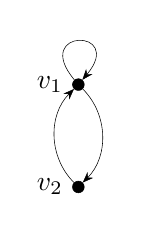
\begin{tikzpicture}[node distance={13mm}, very thin, main/.style = {draw, circle, fill, inner sep=1.5pt, minimum size=0pt}] 
                \node[main] (1) [label=left:$v_1$]{}; 
                \node[main] (2) [below of=1]
                [label=left:$v_2$]{};

            \draw[-Stealth] (1) to [bend left =45](2); 
            \draw[-Stealth] (2) to [bend left =45] (1); 
            \draw[-Stealth] (1) to [out=130,in=50,looseness=22] (1);
        \end{tikzpicture}
    %\caption*{$(a)$}
\end{minipage}
\begin{minipage}[b]{0.23\linewidth}
    \centering
      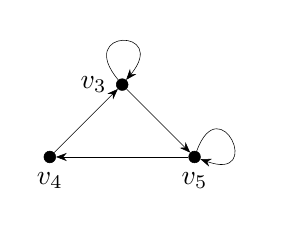
\begin{tikzpicture}[node distance={13mm}, very thin, main/.style = {draw, circle, fill, inner sep=1.5pt, minimum size=0pt}] 
                \node[main] (1) [label=left:$v_3$]{}; 
                \node[main] (2) [below left of=1]
                [label=below :$v_4$]{};
                \node[main] (3) [below right of=1][label=below:$v_5$]{};

            \draw[-Stealth] (1) -- (3);
            \draw[-Stealth] (3) -- (2); 
            \draw[-Stealth] (2) -- (1);             
            \draw[-Stealth] (1) to [out=130,in=50,looseness=22] (1);
            \draw[-Stealth] (3) to [out=70,in=-20,looseness=20] (3);  
        \end{tikzpicture}
    %\caption*{$(b)$}
\end{minipage}
\caption{$D_S=\overleftrightarrow{K_2^+} \cup (\overrightarrow{C_3})_{S'}$.}
\end{figure}

Nevertheless, we have the following result.
	\begin{proposition}
		Let $D_S$ be a digraph of order $n$ and $\sigma$ self-loops. Let $D_i, 1 \leq i \leq k,$ be its strong components, each with order $n_i$ and $\sigma_i$ self-loops. Then
		$$\left|E(D_S)-\sum_{i=1}^k E(D_i) \right| \leq 2\sigma.$$
	\end{proposition}
	
	\begin{proof}
		 For fixed $i$, using the triangle inequality,
		\begin{align}\label{streq:1}
			\sum_{j=1}^{n_i} \left| \Re(\lambda_{i,j})\right|
			&= \sum_{j=1}^{n_i} \left| \Re(\lambda_{i,j})-\frac{\sigma}{n} + \frac{\sigma}{n}  \right| \nonumber\\
			&\leq \sum_{j=1}^{n_i} \left( \left| \Re(\lambda_{i,j})-\frac{\sigma}{n}  \right| + \left| \frac{\sigma}{n}  \right| \right) \nonumber \\
			&= \sum_{j=1}^{n_i} \left| \Re(\lambda_{i,j})-\frac{\sigma}{n}  \right| + \frac{\sigma}{n}n_i.
		\end{align}
		
		On the other hand, using the reverse triangle inequality,
		\begin{align}\label{streq:2}
			\sum_{j=1}^{n_i} \left| \Re(\lambda_{i,j})\right| &= \sum_{j=1}^{n_i} \left| \Re(\lambda_{i,j})-\frac{\sigma_i}{n_i} + \frac{\sigma_i}{n_i}  \right|\nonumber \\
			&\geq \sum_{j=1}^{n_i} \left( \left| \Re(\lambda_{i,j})-\frac{\sigma_i}{n_i}  \right| - \left| \frac{\sigma_i}{n_i} \right| \right) \nonumber\\
			&=E(D_i) - \sigma_i.
		\end{align}
		Summing \eqref{streq:1} and \eqref{streq:2} over all $i,$  we obtain
		\begin{align*}
			E(D_S)+\sigma 
%			&=\sum_{i=1}^k \left[ \sum_{j=1}^{n_i} \left| \Re(\lambda_{i,j})-\frac{\sigma}{n}  \right| + \frac{\sigma}{n}n_i \right ]\\
			&\geq \sum_{i=1}^k \sum_{j=1}^{n_i} \left| \Re(\lambda_{i,j})\right|
			\geq \sum_{i=1}^k \left[ E(D_i) - \sigma_i \right] 
			= \sum_{i=1}^k E(D_i) - \sigma.
		\end{align*}
		Hence, 
		\[
		E(D_S) -\sum_{i=1}^k E(D_i) \geq -2\sigma.
		\]
		By replacing $\dfrac{\sigma}{n}$ with $\dfrac{\sigma_i}{n_i}$ (and vice versa) in each inequality, we have 
		\[
		2\sigma \geq E(D_S) -\sum_{i=1}^k E(D_i).
		\]
		Therefore, 
		\[
		\left|E(D_S)-\sum_{i=1}^k E(D_i) \right| \leq 2\sigma. \qedhere
		\]  
	\end{proof}

The following theorem features a necessary condition on when the energy of a digraph with self-loops is less than or equal to the sum of energies of its strong components:

\begin{theorem}\label{suffcond1}
	Suppose $D_S$ is a digraph of order $n$ with $\sigma$ self-loops. Let $D_i, 1 \leq i \leq k,$ be its strong components, each with order $n_i$ and $\sigma_i$ self-loops, such that $n=\sum_{i=1}^k n_i$ and $\sigma=\sum_{i=1}^k \sigma_i$. Let $1\leq l <k$. Suppose $\frac{\sigma_i}{n_i} > \frac{\sigma}{n}$ holds for $i=1, \ldots, l$ and $\frac{\sigma_i}{n_i} \leq \frac{\sigma}{n}$ holds for $i=l+1, \ldots, k$. Let 
	\begin{align*}
	A_i &=\left\{ j\in[n_i] :      \Re(\lambda_{i,j})> \frac{\sigma}{n}\right\}, \\
        B_i &=\left\{ j\in[n_i] : \Re(\lambda_{i,j})> \frac{\sigma_i}{n_i} \right\}.
	\end{align*}  
    Then the following implication
    \begin{equation*}
        \sum_{i=1}^l \left( \frac{\sigma_i}{n_i}-\frac{\sigma}{n}\right) |A_i| \leq \sum_{i=l+1}^k \left( \frac{\sigma}{n}-\frac{\sigma_i}{n_i} \right)|A_i| \implies E(D_S) \leq \sum_{i=1}^k E(D_i)
    \end{equation*}
    holds. Moreover, if the inequality on the left hand side of the implication is strict, then the inequality on the right hand side will also be strict.
\end{theorem}

    Before we start the proof, note that it is impossible for $\frac{\sigma_i}{n_i} < \frac{\sigma}{n}$ to hold for all $i\in [k]$ since this would implies $\sigma=\sum_{i=1}^k \sigma_i < \frac{\sigma}{n}  \sum_{i=1}^k n_i= \sigma$.
	Similarly for $\frac{\sigma_i}{n_i} > \frac{\sigma}{n}$. However, it is possible that $\frac{\sigma_i}{n_i} = \frac{\sigma}{n}$ holds for all $i \in [k]$ (For example, $\frac{n}{2} \widetilde{K_2}$). This justifies the restriction on $l$.

\begin{proof}
	From the definitions of $A_i$ and $B_i,$ we have $B_i \subset A_i$ for $i=1,\ldots,l$ and $A_i \subset B_i$ for $i=l+1, \ldots, k$.
	From equation \eqref{eq_energy_2_times},
	\begin{align*}
	E(D_S)
	&= \sum_{i=1}^k \left[ 2\sum_{j\in A_i} \left( \Re(\lambda_{i,j})-\frac{\sigma}{n} \right) \right]\\
	&= 2\left[\sum_{i=1}^l  \sum_{j\in A_i} \left( \Re(\lambda_{i,j})-\frac{\sigma}{n} \right)  + \sum_{i=l+1}^k  \sum_{j\in A_i} \left( \Re(\lambda_{i,j})-\frac{\sigma}{n} \right) \right]\\
	&= 2 \sum_{i=1}^l  \left[  \left(\sum_{j\in B_i} + \sum_{j\in A_i-B_i}  \right) \left( \Re(\lambda_{i,j}) -\frac{\sigma_i}{n_i} +\frac{\sigma_i}{n_i}-\frac{\sigma}{n} \right) \right] \\
	&\quad + 2\sum_{i=l+1}^k \left[ \sum_{j\in A_i} \left( \Re(\lambda_{i,j})-\frac{\sigma}{n} \right) 
	+\sum_{j\in B_i-A_i} \left( \Re(\lambda_{i,j})-\frac{\sigma}{n} \right)-\sum_{j\in B_i-A_i} \left( \Re(\lambda_{i,j})-\frac{\sigma}{n} \right)\right] \\
	&= 2\sum_{i=1}^l \left[  \sum_{j\in B_i} \left( \Re(\lambda_{i,j}) -\frac{\sigma_i}{n_i}\right) + \sum_{j\in A_i-B_i} \left( \Re(\lambda_{i,j}) -\frac{\sigma_i}{n_i} \right)  + \sum_{j\in A_i} \left( \frac{\sigma_i}{n_i}-\frac{\sigma}{n} \right)   \right]\\
	&\quad+ 2\sum_{i=l+1}^k \left[ \sum_{j\in B_i} \left( \Re(\lambda_{i,j})-\frac{\sigma_i}{n_i} \right) + \sum_{j\in B_i} \left( \frac{\sigma_i}{n_i}-\frac{\sigma}{n} \right)-\sum_{j\in B_i-A_i} \left( \Re(\lambda_{i,j})-\frac{\sigma}{n} \right)  \right],
	\end{align*}

	where the fourth equality follows from
	\begin{align*}
	\sum_{j\in A_i} &\left( \Re(\lambda_{i,j})-\frac{\sigma}{n} \right) 
	+\sum_{j\in B_i-A_i} \left( \Re(\lambda_{i,j})-\frac{\sigma}{n} \right) \\
	&= \sum_{j\in B_i} \left( \Re(\lambda_{i,j})-\frac{\sigma}{n} \right) 
	=\sum_{j\in B_i} \left( \Re(\lambda_{i,j})-\frac{\sigma_i}{n_i} \right) + \sum_{j\in B_i} \left( \frac{\sigma_i}{n_i}-\frac{\sigma}{n} \right).
	\end{align*}
	Since $\sum_{i=1}^k E(D_i)= 2 \left[\sum_{i=1}^l  \sum_{j\in B_i} \left( \Re(\lambda_{i,j}) -\frac{\sigma_i}{n_i}\right) +  \sum_{i=l+1}^k  \sum_{j\in B_i} \left( \Re(\lambda_{i,j})-\frac{\sigma_i}{n_i} \right) \right],$ we have
	\begin{align*}
	E(D_S) 
	&= \sum_{i=1}^k E(D_i) + 2\sum_{i=1}^l  \sum_{j\in A_i-B_i} \left( \Re(\lambda_{i,j}) -\frac{\sigma_i}{n_i} \right) + 2\sum_{i=1}^l \left( \frac{\sigma_i}{n_i}-\frac{\sigma}{n} \right) |A_i| \\
	&\hspace{-2em} + 2\sum_{i=l+1}^k \left( \frac{\sigma_i}{n_i}-\frac{\sigma}{n} \right) |B_i| - 2\sum_{i=l+1}^k \sum_{j\in B_i-A_i} \left( \Re(\lambda_{i,j}) -\frac{\sigma_i}{n_i}\right) - 2\sum_{i=l+1}^k \sum_{j\in B_i-A_i} \left( \frac{\sigma_i}{n_i}-\frac{\sigma}{n}\right).
	\end{align*}	
	For $i=1,\ldots,l$ and $j\in A_i-B_i, \frac{\sigma}{n}< \Re(\lambda_{i,j}) \leq \frac{\sigma_i}{n_i}$. So $2\sum_{i=1}^l  \sum_{j\in A_i-B_i} \left( \Re(\lambda_{i,j}) -\frac{\sigma_i}{n_i} \right) \leq 0$. Similarly, $-2\sum_{i=l+1}^k \sum_{j\in B_i-A_i} \left( \Re(\lambda_{i,j}) -\frac{\sigma_i}{n_i}\right) \leq 0$. Thus,   
	\begin{align*}
	E(D_S)
	&\leq \sum_{i=1}^k E(D_i)+0 + 2\sum_{i=1}^l \left( \frac{\sigma_i}{n_i}-\frac{\sigma}{n} \right) |A_i|\\
	&\quad + 2\sum_{i=l+1}^k \left( \frac{\sigma_i}{n_i}-\frac{\sigma}{n} \right) |B_i|+0 - 2\sum_{i=l+1}^k \left( \frac{\sigma_i}{n_i}-\frac{\sigma}{n} \right) [|B_i|-|A_i|]\\
	&=\sum_{i=1}^k E(D_i) + 2\sum_{i=1}^l \left( \frac{\sigma_i}{n_i}-\frac{\sigma}{n} \right)|A_i|+ 2\sum_{i=l+1}^k \left( \frac{\sigma_i}{n_i}-\frac{\sigma}{n} \right) |A_i|.
	\end{align*}
	By our assumption, $\sum_{i=1}^l \left( \frac{\sigma_i}{n_i}-\frac{\sigma}{n} \right)|A_i|+ \sum_{i=l+1}^k \left( \frac{\sigma_i}{n_i}-\frac{\sigma}{n} \right) |A_i|\leq 0$. Therefore, $E(D_S) \leq \sum_{i=1}^k E(D_i)$.
\end{proof}

The next theorem provides a necessary condition for $E(D_S)\leq \sum_{i=1}^k E(D_i)$ to hold.

\begin{theorem}
    With the same assumption as in Theorem \ref{suffcond1}. The following implication  
    \begin{equation*}
        E(D_S)\leq \sum_{i=1}^k E(D_i) \implies \sum_{i=1}^l \left( \frac{\sigma_i}{n_i}-\frac{\sigma}{n} \right)|B_i| \leq \sum_{i=l+1}^k \left( \frac{\sigma}{n}-\frac{\sigma_i}{n_i} \right) |B_i|
    \end{equation*}
    holds. If the inequality on the left-hand side of the implication is strict, then the inequality on the right-hand side will also be strict.
\end{theorem}

\begin{proof}
    For $i=1,\ldots,l$, we have $\frac{\sigma_i}{n_i}-\frac{\sigma}{n}> 0$  and $\frac{\sigma_i}{n_i}-\frac{\sigma}{n} \leq 0$ for $i=l+1,\ldots,k$. Note that	
	\begin{align*}
			&E(D_S)-\sum_{i=1}^k E(D_i)\\
			&= 2   \sum_{i=1}^l \sum_{j\in A_i} \left( \Re(\lambda_{i,j})-\frac{\sigma}{n} \right)  + 2\sum_{i=l+1}^k  \sum_{j\in A_i} \left( \Re(\lambda_{i,j})-\frac{\sigma}{n} \right) \\
			&\qquad - 2\sum_{i=1}^l \sum_{j\in B_i} \left( \Re(\lambda_{i,j})-\frac{\sigma_i}{n_i} \right)  - 2\sum_{i=l+1}^k \sum_{j\in B_i} \left( \Re(\lambda_{i,j})-\frac{\sigma_i}{n_i} \right)\\
			&= 2\sum_{i=1}^l \sum_{j\in A_i-B_i} \left( \Re(\lambda_{i,j})-\frac{\sigma}{n} \right) + 2\sum_{i=1}^l \sum_{j\in B_i} \left( \Re(\lambda_{i,j})-\frac{\sigma}{n} \right)  + 2\sum_{i=l+1}^k \sum_{j\in A_i} \left( \Re(\lambda_{i,j})-\frac{\sigma}{n} \right) \\
			& -2\sum_{i=1}^l \sum_{j\in B_i} \left( \Re(\lambda_{i,j})-\frac{\sigma_i}{n_i} \right)  - 2\sum_{i=l+1}^k \sum_{j\in B_i-A_i} \left( \Re(\lambda_{i,j})-\frac{\sigma_i}{n_i} \right)  - 2\sum_{i=l+1}^k \sum_{j\in A_i} \left( \Re(\lambda_{i,j})-\frac{\sigma_i}{n_i} \right)\\
			&= 2\sum_{i=1}^l \sum_{j\in A_i-B_i} \left( \Re(\lambda_{i,j})-\frac{\sigma}{n} \right)  + 2\sum_{i=1}^l \sum_{j\in B_i}\left(\frac{\sigma_i}{n_i}-\frac{\sigma}{n} \right)
			- 2\sum_{i=l+1}^k\sum_{j\in B_i-A_i} \left( \Re(\lambda_{i,j}) -\frac{\sigma_i}{n_i} \right) \\ 
			&\qquad+  2\sum_{i=l+1}^k \sum_{j\in A_i} \left(\frac{\sigma_i}{n_i}-\frac{\sigma}{n} \right)\\
			&= 2\sum_{i=1}^l \sum_{j\in A_i-B_i} \left( \Re(\lambda_{i,j})-\frac{\sigma}{n} \right)  + 2\sum_{i=1}^l \sum_{j\in B_i}\left(\frac{\sigma_i}{n_i}-\frac{\sigma}{n} \right) 
			- 2\sum_{i=l+1}^k \sum_{j\in B_i-A_i} \left( \Re(\lambda_{i,j})-\frac{\sigma}{n} \right) \\
			&\qquad + 2\sum_{i=l+1}^k \sum_{j\in B_i-A_i}\left(\frac{\sigma_i}{n_i}-\frac{\sigma}{n} \right)  + 2\sum_{i=l+1}^k \sum_{j\in A_i}\left(\frac{\sigma_i}{n_i}-\frac{\sigma}{n} \right).
	\end{align*}
	Since 
	\[
	E(D_S)-\sum_{i=1}^k E(D_i) \leq 0
	\]
	and 
	\[
	2\sum_{i=1}^l \sum_{j\in A_i-B_i} \left( \Re(\lambda_{i,j})-\frac{\sigma}{n} \right)  - 2\sum_{i=l+1}^k \sum_{j\in B_i-A_i} \left( \Re(\lambda_{i,j})-\frac{\sigma}{n} \right)  \geq 0,
	\] we have 
	\[
	2\sum_{i=1}^l \sum_{j\in B_i}\left(\frac{\sigma_i}{n_i}-\frac{\sigma}{n} \right)  + 2\sum_{i=l+1}^k \sum_{j\in B_i-A_i}\left(\frac{\sigma_i}{n_i}-\frac{\sigma}{n} \right)  + 2\sum_{i=l+1}^k \sum_{j\in A_i}\left(\frac{\sigma_i}{n_i}-\frac{\sigma}{n} \right) \leq 0.
	\] 
	Therefore $\sum_{i=1}^l \left( \frac{\sigma_i}{n_i}-\frac{\sigma}{n} \right)|B_i| \leq \sum_{i=l+1}^k \left( \frac{\sigma}{n}-\frac{\sigma_i}{n_i} \right) |B_i|$.
\end{proof}

\begin{remark}
	Observe that 
	\begin{align*}
		&\sum_{i=1}^l \left( \frac{\sigma_i}{n_i}-\frac{\sigma}{n}\right) |A_i| - \sum_{i=l+1}^k \left( \frac{\sigma}{n}-\frac{\sigma_i}{n_i} \right)|A_i|\\
		&=\sum_{i=1}^l \left( \frac{\sigma_i}{n_i}-\frac{\sigma}{n} \right)|B_i| - \sum_{i=l+1}^k \left( \frac{\sigma}{n}-\frac{\sigma_i}{n_i} \right) |B_i| + \sum_{i=1}^l \left( \frac{\sigma_i}{n_i}-\frac{\sigma}{n} \right)\left(|A_i|-|B_i| \right) \\
		& \quad+ \sum_{i=l+1}^k \left( \frac{\sigma}{n}-\frac{\sigma_i}{n_i} \right) \left(|B_i|-|A_i|\right).
	\end{align*}
	Since the last two terms are greater or equals to zero, we have 
	\[
	\sum_{i=1}^l \left( \frac{\sigma_i}{n_i}-\frac{\sigma}{n}\right) |A_i| - \sum_{i=l+1}^k \left( \frac{\sigma}{n}-\frac{\sigma_i}{n_i} \right)|A_i|
	\geq \sum_{i=1}^l \left( \frac{\sigma_i}{n_i}-\frac{\sigma}{n} \right)|B_i| - \sum_{i=l+1}^k \left( \frac{\sigma}{n}-\frac{\sigma_i}{n_i} \right) |B_i|.
	\]
\end{remark}

The following lemma generalizes \cite[Proposition 2.1]{rada2009mcclelland}.
 \begin{lemma}
	\label{E(D_S)=0_acyclic}
        Let $D_S$ be a digraph with $\sigma$ self-loops.
	Then $E(D_S)=0$ if and only if $D_S$ is an acyclic digraph with either $\sigma=0$ or $\sigma=n$.
\end{lemma}

\begin{proof}
	The sufficient condition can be shown by direct calculation. We prove the necessary condition.
	Suppose $E(D_S)=0$. Then $\Re(\lambda_i)=\frac{\sigma}{n}$ for all $i=1,\ldots,n$. From $|\Re(\lambda_i)| \leq |\lambda_i| \leq \rho$, this implies $\lambda_i=\frac{\sigma}{n}$ for all $i=1,\ldots,n$. By Lemma \ref{rationalrootsofmonic}, $\frac{\sigma}{n}$ must be an integer. So, $\sigma=0$ or $\sigma=n$. For $\sigma=0$, Rada \cite[Proposition 2.1]{rada2009mcclelland} showed that $D_S=D$ is acyclic. We focus on the case $\sigma=n$. Then $\lambda_i=1$ for all $i$. From $\sum_{i=1}^n \lambda^k_i=w_k$, we have $w_k=n$ for $k \geq 1$. If we exclude the closed walks that consist of just one vertex (in this case, there are $\sigma=n$ of them), then we get that the number of all other possible closed walks is zero. In particular, there is no cycle with length at least two. So $D_S$ is an acyclic digraph with full loops.
\end{proof}

%%%%%%%%%%%%%%%%%%%%%%%%%%%%%%%%%%%%%%%%%%%%%%%%%%
\section{McClelland type bound for the energy of digraphs with self-loops}
\label{sec4}
%%%%%%%%%%%%%%%%%%%%%%%%%%%%%%%%%%%%%%%%%%%%%%%%%%

In this section, we present the McClelland type bound for the energy of digraphs with self-loops, which generalizes \cite[Theorem 2.3]{rada2009mcclelland}: if $\sigma=0,$ then $E(D)\leq \sqrt{ \frac{1}{2}n \left ( m+c_2\right) }.$ 
	

\begin{theorem}
	\label{E(D_S)_leq_sqrt}
	Suppose $D_S$ is a digraph of order $n$, size $m$, $c_2$ 2-cycles, and $\sigma$ self-loops. Then,
	\begin{equation}
		\label{energyinsqrt}
		E(D_S)\leq \sqrt{ \frac{1}{2}n \left ( m+c_2+ 2\sigma-\frac{2\sigma^2}{n} \right) }.
	\end{equation}
	The equality holds if and only if $D_S$ is 
        \begin{enumerate}[(i)]
            \item $ n\overleftrightarrow{K_1} \text{ or } \frac{n}{2} \overleftrightarrow{K_2}.$
            \item $\frac{n}{2}\overleftrightarrow{K_1} \bigcup \frac{n}{2}\widetilde{K_1} \text{ or } \frac{n}{2}\overleftrightarrow{K_2^+}$,
            where $\overleftrightarrow{K_2^+}$ is symmetrization of the complete graph $K_2$ with one self-loop. 
            \item$\frac{n}{2}\widetilde{K_2}$.
        \end{enumerate}
\end{theorem}

\begin{proof}
    By the Cauchy-Schwarz inequality 
    \begin{align*}
         \sum_{i=1}^n a_ib_i \leq \sqrt{\sum_{i=1}^n a_i^2} \sqrt{\sum_{i=1}^n b_i^2},
    \end{align*}
    with $a_i=1$ and $b_i= \left | \Re(\lambda_i)-\frac{\sigma}{n} \right|,$ we obtain
	\begin{align*}    
		E(D_S)
		&= \sum_{i=1}^n \left | \Re(\lambda_i)-\frac{\sigma}{n} \right| \\          
		&\leq \sqrt{n} \sqrt{\sum_{i=1}^n \left | \Re(\lambda_i)-\frac{\sigma}{n} \right|^2} \\      
		&= \sqrt{n} \sqrt{\sum_{i=1}^n \Re(\lambda_i)^2+\frac{\sigma^2}{n}-\frac{2\sigma}{n} \sum_{i=1}^n \Re(\lambda_i)} \\
		&\leq \sqrt{n} \sqrt{ \frac{1}{2}(m+c_2+2\sigma)-\frac{\sigma^2}{n} } \\
		&= \sqrt{ \frac{1}{2}n \left ( m+c_2+ 2\sigma-\frac{2\sigma^2}{n} \right) }.         
	\end{align*}    
    The sufficient condition can be checked by direct computation. We focus on the necessary condition. 

    Firstly, we show that $D_S$ is the direct sum of its strong components. Let $D_S'$ be the sub-digraph of $D_S$ obtained by deleting all the arcs that do not belong to any cycle. By \ref{charpoly_arc_deletion}, we have $\phi(D_S')=\phi(D_S)$. Let $m'$ be the number of arcs of $D_S'$. Then
    \begin{equation*}
        \sqrt{ \frac{1}{2}n \left ( m+c_2+ 2\sigma-\frac{2\sigma^2}{n} \right)}=E(D_S)=E(D_S') \leq \sqrt{ \frac{1}{2}n \left ( m'+c_2+ 2\sigma-\frac{2\sigma^2}{n} \right)}.
    \end{equation*} 
    Solving this gives us $m \leq m'$. Thus $m=m'$. Hence, $D_S$ does not contain any arc that does not belong to a cycle. Now consider any two strong components of $D_S$, say $D_1$ and $D_2$. For any two vertices $v\in D_1$ and $w\in D_2$, if there is an arc joining $v$ and $w$, say $(v,w)$ and $(v,w)$ belongs to a cycle, say $(v,w,v_1, \dots, v_{l},v)$. Then this implies that $v$ is reachable from $w$, contradicting the maximality of $D_1$. Thus, such an arc cannot possibly exist. %by what we shown just now. 
    Therefore, $D_S$ is the disjoint union of its strong components.
   
    Now suppose the equality holds. For all $i=1,...,n$, it holds that $\left | \Re(\lambda_i)-\frac{\sigma}{n} \right|=r$ for some $r\in \mathbb{R}$. So, $\Re(\lambda_i)$ equals to either $\frac{\sigma}{n}+r$ or $\frac{\sigma}{n}-r$. Let $l$ be the number of $\lambda_i$ such that $\Re(\lambda_i)=\frac{\sigma}{n}+r$. From $\sum_{i=1}^n \Re(\lambda_i)=\sigma$, we have 
    \[
    l\left( \frac{\sigma}{n}+r \right) + (n-l) \left( \frac{\sigma}{n}-r \right) = \sigma.
    \]
    Solving this equation gives $2rl = rn.$
	
\begin{enumerate}
	\item Case 1: $r=0$. Then $E(D_S)=0$. By Lemma \ref{E(D_S)=0_acyclic}, $D_S$ is an acyclic digraph with no loop or full loops. In both of the cases,  we have $m=0$ from equality \eqref{energyinsqrt},. This implies that $D_S=n\overleftrightarrow{K_1}$ or $n\widetilde{K_1}$.

	\item Case 2: $r\neq 0$. Then, half of the eigenvalues have real part equal to $\frac{\sigma}{n}+r$ and the other half have real part equal to $\frac{\sigma}{n}-r$. Without loss of generality, we assume $\rho = \frac{\sigma}{n}+r$.
		\begin{enumerate}
			\item Subcase 2.1: All eigenvalues are real. Thus the spectrum of $D_S$ is 
			\begin{center}
				$\text{Spec($D_S$)}= \left\{  \left[\frac{\sigma}{n}+r \right] ^{\frac{n}{2}}, \left[ \frac{\sigma}{n}-r \right]^{\frac{n}{2}} \right\}.$
				
			\end{center}
            
			Subcase 2.1.1: $D_S$ contains $\overleftrightarrow{K_1}$ or $\widetilde{K_1}$. This implies that $\frac{\sigma}{n}+r = 0 \text{ or } 1$. The case $\frac{\sigma}{n}+r = 0$ is impossible since $r>0$.
			
			For $\frac{\sigma}{n}+r=1$, the spectrum of $D_S$ becomes 
			\begin{center}
				$\text{Spec($D_S$)}= \left\{  \left[1 \right] ^{\frac{n}{2}}, \left[ \frac{2\sigma}{n}-1 \right]^{\frac{n}{2}} \right\}.$
			\end{center}
			By Lemma \ref{rationalrootsofmonic}, $\frac{2\sigma}{n}-1$ must be an integer. This only happens when $\sigma = 0, \frac{n}{2} \text{ or } n$.
			\begin{enumerate}[i.]
				\item  If $\sigma=0$. From the spectrum of $D_S$, 
                \begin{center}
				$\text{Spec($D_S$)}= \left\{  \left[1 \right] ^{\frac{n}{2}}, \left[ -1 \right]^{\frac{n}{2}} \right\},$
			\end{center}
               we deduce that it is impossible to contain any isolated vertex $\overleftrightarrow{K_1}$.
                
				\item If $\sigma=\frac{n}{2}$, then $m=c_2=0$ from Equality \eqref{energyinsqrt}. So $D_S=\frac{n}{2} \overleftrightarrow{K_1} \bigcup \frac{n}{2} \widetilde{K_1}$.
                
				\item If $\sigma =n$, then $m=c_2=0$ from Equality \eqref{energyinsqrt}. So, $D_S=n\widetilde{K_1}$.
			\end{enumerate}
			Therefore, $D_S=\frac{n}{2} \overleftrightarrow{K_1} \bigcup \frac{n}{2} \widetilde{K_1} \text{ or }n\widetilde{K_1}$.\\
			
			Subcase 2.1.2: $D_S$ does not contain $\overleftrightarrow{K_1}$ or $\widetilde{K_1}$. Suppose $D_1,\ldots, D_k$ are the strong components of $D_S$, each with order $n_i$ and $\sigma_i$ self-loops. Since $D_S$ has only two distinct eigenvalues, all the strong components of $D_S$ must be identical. Thus $\sigma_1=\cdots=\sigma_k$ and $n_1=\cdots=n_k$. As each strong component $D_i$ has two distinct eigenvalues, by \cite[Corollary 3.5]{cavers2025distinct}, we have the following cases:
            \begin{enumerate}[(i)]
                \item $\sigma_i=0$ and $D_i=\overleftrightarrow{K_{n_i}}$ with spectrum $\{[n_i-1]^1,[-1]^{n_i-1} \}$. We have $\sigma=0$.
                Solving 
                \begin{align*}
                    \frac{\sigma}{n}+r &= n_i-1, \\
                    \frac{\sigma}{n}-r &= -1,
                \end{align*}
            yields $n_i=2$. From $\sum_{i=1}^k n_i=n$, it follows that $k=\frac{n}{2}$. Therefore, $D_S=\frac{n}{2} \overleftrightarrow{K_2}$.

                \item $\sigma_i=1$ and $D_i=\overleftrightarrow{K_2^+}$ with spectrum $\{ [\frac{1}{2}(1+\sqrt{5})]^1, [\frac{1}{2}(1-\sqrt{5})]^1 \}$. We have $\sigma=\sum_{i=1}^k \sigma_i = k$. 
                Solving 
                \begin{align*}
                    \frac{k}{n}+r &=\frac{1}{2}(1+\sqrt{5}), \\
                    \frac{k}{n}-r &=\frac{1}{2}(1-\sqrt{5}),
                \end{align*}
                gives $k=\frac{n}{2}$. Therefore, $D_S=\frac{n}{2}\overleftrightarrow{K_2^+}$.

                \item $2\leq\sigma_i\leq n_i-1$ and $\text{Spec}(D_i)=\{[\sigma_i]^1, [0]^{n_i-1}\}$. Using the same argument, it can be shown that $n_i=2$, which is a contradiction. 

                \item $\sigma_i=n_i$ and $D_i=\widetilde{K_{n_i}}$ with spectrum $\{[n_i]^1, [0]^{n_i-1} \}$. By the same argument, we obtain $n_i=2$ and $k=\frac{n}{2}$. Hence, $D_S=\frac{n}{2}\widetilde{K_2}$.
            \end{enumerate}
        Therefore, $D_S=\frac{n}{2} \overleftrightarrow{K_2}, \frac{n}{2}\overleftrightarrow{K_2^+} \text{ or } \frac{n}{2}\widetilde{K_2}$.\\

	\item Subcase 2.2: The eigenvalues with $\Re(\lambda_i)=\frac{\sigma}{n}-r$ and $\Im(\lambda_i) \neq 0$ for some $i$. We show that this case is impossible. Observe that in this case, the spectrum of $D_S$ becomes
	\begin{center}
				$\text{Spec($D_S$)}= \left\{  \left[\dfrac{\sigma}{n}+r \right] ^{\frac{n}{2}}, \underbrace{\frac{\sigma}{n}-r + i\Im(\lambda_k) }_{\frac{n}{2} \text{ times} }\right\}.$
				
			\end{center}
	
        By a simple computation, we get
%5$r=\sqrt{\frac{1}{2n}(m+c_2+2\sigma-\frac{2\sigma^2}{n})}$ and 
        \begin{align*}
            \sum_{k=1}^{\frac{n}{2}} \Im(\lambda_k)^2=\frac{m-c_2}{2}.
        \end{align*}
        By our assumption, we have $m>c_2$. First, we show that $D_S$ could not possibly contain an isolated vertex (Either with a loop or without a loop). This corresponds to $r=-\frac{\sigma}{n}, 1-\frac{\sigma}{n}, \frac{\sigma}{n}, \text{ or } \frac{\sigma}{n}-1$. The cases of $r=-\frac{\sigma}{n}$ and $\frac{\sigma}{n}-1$ are impossible as $r>0$. Thus, we are left with only two cases, i.e. $r=\frac{\sigma}{n}$ or $1-\frac{\sigma}{n}$.
        
        \begin{enumerate}[(i)]
            \item Case 1: $r=\frac{\sigma}{n}$. 
            
            Then $\frac{2\sigma}{n}$ is a root of $\phi(\lambda)$. So it must be an integer. So $\sigma=0, \frac{n}{2}$ or $n$.
            From 
            \begin{equation*}
                r=\sqrt{\frac{1}{2n} \left( m+c_2+2\sigma-\frac{2\sigma^2}{n} \right)},
            \end{equation*}
             we have $m+c_2=0$ for all cases, which contradicts our assumption $m>c_2$. This means that $D_S$ cannot possibly contain an isolated vertex $\overleftrightarrow{K_1}$. 
            
            \item Case 2: $r=1-\frac{\sigma}{n}$. 
            
            If there exists at least one purely real eigenvalue $\frac{\sigma}{n}-r$, then $\sigma=0,\frac{n}{2}$ or $n$, but this again gives $m+c_2=0$. So all eigenvalues with $\Re(\lambda_k)=\frac{\sigma}{n}-r$ must be complex. Each complex number must be in some spectrums that contains at least one $\frac{\sigma}{n}+r$ (Since each strong component must have at least one nonnegative real eigenvalue and the only possible candidate is $\frac{\sigma}{n}+r$). Therefore, $D_S$ cannot possibly contains $\widetilde{K_1}$ too.
        \end{enumerate}
     
     This implies that the spectrum of each strong component of $D_S$ must necessarily contains at least two eigenvalues. Moreover, $D_S$ has at least $\frac{n}{2}$ strong components. This means that every eigenvalue equals to $\frac{\sigma}{n}+r$ must be in a spectrum that contains at least one eigenvalue with real part equals to $\frac{\sigma}{n}-r$. This is only possible if and only if all eigenvalues are real, contradicting our assumption that there exists some complex eigenvalues. Thus, all eigenvalues must be real.
    \end{enumerate}
\end{enumerate}
\end{proof}


%%%%%%%%%%%%%%%%%%%%%%%%%
\section{Some Bounds For Spectral Radius Of Digraphs With Self-Loops And Its Complement}
\label{sec5}
%%%%%%%%%%%%%%%%%%%%%%%%%
    In this section, we define the complement of a digraph with self-loops $D_S$ and give a few bounds for the spectral radius of $D_S$ and its complement. We first recall some definitions that will be frequently used throughout this section.

    \begin{definition} \cite{kolotilina1993perronroot}
        Let $A$ be an $n\times n$ real matrix such that $a_{ij}a_{ji}\geq0$ for all $1\leq i,j \leq n$. The geometric symmetrization of $A$ is a matrix $S(A)=(s_{ij})$ such that $s_{ij}=\sqrt{a_{ij}a_{ji}}.$ Clearly, $S(A)$ is symmetric and if $A$ is symmetric, then $A=S(A)$.
    \end{definition}

    \begin{definition}
    \cite{kolotilina1993perronroot}    
    Let $A$ and $B$ be $n\times n$ real matrices. Then, $A$ is said to be diagonally similar to $B$, denoted as $A \overset{D}{\sim} B$, if there exists a real diagonal matrix $D=Diag(d_1, \ldots, d_n)$ such that $A=D^{-1}BD$.
    \end{definition}

    For an $(0,1)$-matrix $A$, we have the following result:

    \begin{lemma}
        \label{A_diagonal similar_SA}
        Suppose $A$ is an $(0,1)$-matrix and $A$ is diagonally similar to $S(A)$. Then, $A$ is symmetric. 
    \end{lemma}

    \begin{proof}
        Since $A \overset{D}{\sim} S(A)$, we have $DAD^{-1}=S(A)$. This implies $\frac{d_i}{d_j}a_{ij}=\sqrt{a_{ij}a_{ji}}$. Suppose $a_{ij}\neq a_{ji}$. Without loss of generality, assume $a_{ij}=1$ and $a_{ji}=0.$ Then, $\frac{d_i}{d_j}=0$, which is impossible as $d_i,d_j\neq 0$. Thus, $a_{ij}=a_{ji}$ and $A$ is symmetric.
    \end{proof}

    
    The following inequality generalizes the lower bound given in \cite{gudino2010lowerboundofspectral}.
    \begin{lemma}
        \label{lemmalowerbound_p}
        Let $A$ be the adjacency matrix of a digraph $D_S$ of order $n$, $c_2$ $2$-cycles, and $\sigma$ self-loops. Let $\rho(A)$ be the spectral radius of $A$. Then, 
        \begin{equation}
            \label{eqlowerbound_p}
            \rho(A) \geq \frac{c_2+\sigma}{n}.
        \end{equation}        
        The equality holds if and only if $D_S=\overleftrightarrow{G_S}+ \text{\{Some arcs that do not belong to cycles\}}$, where $G_S$ is a $(\frac{c_2+\sigma}{n},\frac{c_2+\sigma}{n}+1) $-bidegreed graph with self-loops such that
        \begin{align*}
            deg_{G_S}(v)= 
            \begin{cases}
	\frac{c_2+\sigma}{n}+1, &\text{if $v\in S$} ,\\
	\frac{c_2+\sigma}{n}, &\text{if $v \in \cV-S$. }
            \end{cases}
        \end{align*}
    \end{lemma}

    \begin{proof}
        By \cite[Theorem 1]{kolotilina1993perronroot}, we have $\rho(A)\geq \rho(S(A))$. Let $j=(1, \ldots, 1)^T$. Using the Rayleigh quotient for $S(A)$, we have 
        \begin{align*}
            \rho(A) &\geq \rho(S(A))\\
            &=\max_{v\in \R^n-\{0\}} \frac{v^TS(A)v}{v^Tv}\\
            &\geq \frac{j^TS(A)j}{j^Tj}\\
            &=\frac{c_2+\sigma}{n}.
        \end{align*}
        
        Suppose the equality holds. Let $D_S$ be the disjoint union of its strong components, $D_1, \ldots, D_k$, with adjacency matrices $A_1, \ldots, A_k$ respectively. So,
        \begin{equation}
        A=\begin{bmatrix}
        
            A_1 &        &0    \\
               & \ddots                \\
            0    &        & A_k
        \end{bmatrix}.
        \end{equation}
        By \cite[Theorem 2]{kolotilina1993perronroot}, each $A_i$ is diagonally similar to $S(A_i)$ and $S(A_i)j=\rho(A)j$ for every $i$. By Lemma \ref{A_diagonal similar_SA}, each $A_i$ is symmetric. Thus, we conclude that $D_S$ is symmetric and there is a graph with self-loops $G_S$ such that $D_S=\overleftrightarrow{G_S}$.
        Since $D_S$ is symmetric, we have 
        $$deg^+(v_i)=deg^-(v_i)=\sum_{j=1}^n a_{ij}=\sum_{j=1}^n s_{ij}=\rho(A)=\frac{c_2+\sigma}{n}.$$
        Therefore, we conclude that $D_S=\overleftrightarrow{G_S}$ is $\frac{c_2+\sigma}{n}$-regular.

        Now if $D_S$ contains $D_1, \ldots, D_k$ strong components but not necessary disjoint union of them, by deleting all the arcs that do not belong to any cycle and applying the above argument, we conclude that $D_S=\overleftrightarrow{G_S}+ \text{\{Some arcs that do not belong to cycles\}}$.
    \end{proof}
    
    Next, we give a lower bound of $E(D_S)$ in terms of $c_2$ and $n$. 
    \begin{lemma}
    \label{lemma_lower_bound_E(D_S)_c_2}
        Let $D_S$ be a digraph of order $n$, $c_2$ $2$-cycles and $\sigma$ self-loops. Then, 
        \begin{equation}
        \label{lowerbound_E(D_S)c_2}
            E(D_S)\geq \frac{2c_2}{n}. 
        \end{equation}
        The equality holds if and only if $D_S=\overleftrightarrow{G_S}+ \text{\{Some arcs that do not belong to cycles\}}$, where  $G_S$ is a $(\frac{c_2+\sigma}{n},\frac{c_2+\sigma}{n}+1) $-bidegreed graph with self-loops such that
        \begin{align*}
            deg_{G_S}(v)= 
            \begin{cases}
	\frac{c_2+\sigma}{n}+1, &\text{if $v \in S$},\\
	\frac{c_2+\sigma}{n}, &\text{if $v \in \cV-S$. }
    \end{cases}
        \end{align*}
    \end{lemma}

    \begin{proof}
        The inequality follows easily from 
        \begin{equation}
            \label{longineqofE(D_S)_2c_2_n}
            E(D_S)=2\sum_{\Re(\lambda_i) > \frac{\sigma}{n}} \left( \Re(\lambda_i)-\frac{\sigma}{n} \right) \geq 2 \left(\rho-\frac{\sigma}{n} \right) \geq \frac{2c_2}{n},
        \end{equation}
        where the first equality follows from Proposition \ref{energy+} and the last inequality follows from Lemma \ref{lemmalowerbound_p}. Suppose the equality \eqref{lowerbound_E(D_S)c_2} holds. From \eqref{longineqofE(D_S)_2c_2_n}, it follows that $\rho =\frac{c_2+\sigma}{n}$. By Lemma  \ref{lemmalowerbound_p}, we know $D_S=\overleftrightarrow{G_S}+ \text{\{Some arcs that do not belong to cycles\}}$, where $G_S$ is a $\frac{c_2+\sigma}{n}$-regular graph with self-loops.
    \end{proof}

From the above lemma, we can deduce some digraphs that satisfy the equality.
    \begin{corollary}
        Equality \eqref{lowerbound_E(D_S)c_2} is satisfied if $D_S=\overleftrightarrow{K}_{(\frac{n}{n-\rho}) \times (n-\rho)}, \overleftrightarrow{K_n}, \widetilde{K}_{(\frac{n}{n-\rho}) \times (n-\rho)}$ and $\widetilde{K_n}$, where $\rho=\frac{c_2}{n}$.
    \end{corollary}

    \begin{proof}
        From Lemma \ref{lowerbound_E(D_S)c_2}, we know that all eigenvalues of $D_S$ are real. Consider first $\sigma=0$. So $\rho=\frac{c_2}{n}$. Equality \eqref{longineqofE(D_S)_2c_2_n} implies that $\rho$ is the only positive eigenvalue and $G_S=G$ is $\frac{c_2}{n}$-regular. By \cite[Theorem 3.23]{cvetkovic1995spectra}, $G$ is connected. Suppose further that $D=\overleftrightarrow{G}$.
        
        Assume that $D$ has $0$ as its eigenvalue.
                 Let us further suppose all negative eigenvalues are equal, say $\mu$. The spectrum of $D$ becomes
                 \begin{align*}
                 \mathrm{Spec}(D) =\{[\rho]^1, [0]^f, [\mu]^g \},
                 \end{align*}
                 where $f$ and $g$ are the multiplicities of $0$ and $\mu$, respectively.
                By \cite[Theorem 6.6]{cvetkovic1995spectra}, it follows that $G$ is a complete multi-partite graph $K_{\left(-\frac{\rho}{\mu}+1\right)\times -\mu}$. Let us determine the values of $f,g$ and $\mu$ respectively.
                 
                 From Equality \eqref{longineqofE(D_S)_2c_2_n}, it follows that  
                 \begin{align*}
                  g\mu &=- \rho.
                \end{align*}
                We also have 
                \begin{align*}
                    1+f+g=n,
                \end{align*}
                as the sum of multiplicities of all eigenvalues must be $n$. Moreover, from 
                \begin{align*}
                    \sum_{i=1}^n \lambda_i^2=m=n\rho,
                \end{align*}
                we obtain 
                \begin{align*}
                    g\mu^2=n\rho-\rho^2.
                \end{align*}
                Solving the simultaneous equations gives us 
                \begin{align*}
                    f &= \frac{n(n-\rho-1)}{n-\rho} ,\\
                    g &=\frac{\rho}{n-\rho}, \\
                    \mu &= -(n-\rho). 
                \end{align*}
        Therefore, $D=\overleftrightarrow{K_{(\frac{n}{n-\rho}) \times (n-\rho)}}$. 

%%Moreover, $G$ is a strongly regular graph with parameters $(n,d,2d-n,d)$.  

        On the other hand, if we assume that the spectrum of $D$ does not contain $0$ as one of its eigenvalues and only have one negative eigenvalue, then the spectrum of $D$ is 
            \begin{align*}
                     \mathrm{Spec}(D) =\{[\rho]^1, [\mu]^g \},
            \end{align*}
        By \cite[Theorem 6.4]{cvetkovic1995spectra}, we conclude that $D= \overleftrightarrow{K_{n}}$.

         Since $E(\widetilde{D})=E(D)$ by Lemma \ref{lemma_E(D_S)=E(D)}, it follows that $\widetilde{K}_{(\frac{n}{n-\rho}) \times (n-\rho)}$ and $\widetilde{K_n}$ also satisfy the equality.
    \end{proof}
    
    Next, we give an upper bound for $\rho$. 
    \begin{lemma}
        \label{lemma_ub_rho}
        Let $D_S$ be a digraph of order $n\geq2$, size $m$, $c_2$ $2$-cycles and $\sigma$ self-loops. Let $\rho$ be the spectral radius of $D_S.$ Then, 
        $$\rho \leq \frac{\sigma}{n} + \sqrt{\frac{\sigma^2}{n^2}-\frac{\sigma^2}{n}+\frac{(n-1)(m+c_2+2\sigma)}{2n}}.$$
        The equality is satisfied if $D_S=\overleftrightarrow{K_n} \text{ and } \widetilde{K_n}$.
    \end{lemma}

    \begin{proof}
    From Lemma \ref{sum_eigenvalue}, we have 
    $$\rho-\sigma=-\sum_{i=2}^n \Re(\lambda_i).$$
    Squaring both sides and apply the Cauchy-Schwarz inequality gives
    \begin{align*}
        (\rho-\sigma)^2= \left( -\sum_{i=2}^n \Re(\lambda_i) \right)^2 \leq (n-1)\sum_{i=2}^n \Re(\lambda_i)^2.
    \end{align*}
    Therefore, 
    \begin{align*}
        \sum_{i=2}^n \Re(\lambda_i)^2 \geq \frac{(\rho-\sigma)^2}{n-1}.
    \end{align*}
    By equation \eqref{eq:ReImineq1},
    \begin{align*}
        c_2+\sigma &= \rho^2 + \sum_{i=2}^n \Re(\lambda_i)^2 - \Im(\lambda_i)^2\\
        &\geq \rho^2 + \frac{(\rho-\sigma)^2}{n-1} - \frac{m-c_2}{2}.
    \end{align*}
    Rearranging and grouping the like terms, we obtain
    \begin{align}
    \label{quadraticrholeq0}
        2n\rho^2-4\sigma\rho+2\sigma^2-(n-1)(m+c_2+2\sigma) &\leq0.
    \end{align}
    The quadratic polynomial $f(\rho)=2n\rho^2-4\sigma\rho+2\sigma^2-(n-1)(m+c_2+2\sigma)$ has roots 
    \begin{align*}
        \rho = \frac{\sigma}{n} \pm \sqrt{\frac{\sigma^2}{n^2}-\frac{\sigma^2}{n}+\frac{(n-1)(m+c_2+2\sigma)}{2n}}.
    \end{align*}
    From inequality \eqref{quadraticrholeq0}, we have 
    \begin{align*}
        \rho \leq \frac{\sigma}{n} + \sqrt{\frac{\sigma^2}{n^2}-\frac{\sigma^2}{n}+\frac{(n-1)(m+c_2+2\sigma)}{2n}}.
    \end{align*}
    The sufficient conditions can be checked by direct computation.
    \end{proof}

    Now we define the complement of digraphs with self-loops and explore some of its properties.
    \begin{definition}
        \label{complement_def}
        Let $D_S$ be a digraph with self-loops with adjacency matrix $A(D_S)$ and $S\neq \emptyset$. The complement of $D_S$, denoted as $\overline{D_S}$ is defined to be $(\overline{D})_{V-S}$. 
        
        In other words, if $A(\overline{D_S})$ is the adjacency of $\overline{D_S}$, then $A(D_S)+A(\overline{D_S})=J_n.$
    \end{definition}

    \begin{remark}
        If a digraph $D$ has zero self-loop, then we have $A(D)+A(\overline{D})=J_n-I_n$. To incorporate this into Definition \ref{complement_def}, define a function $\delta_\sigma: [n] \rightarrow \{0,1\}$ as
        \[\delta_\sigma=
        \begin{cases}
	0, &\text{if } \sigma \neq0,\\
	1, &\text{if } \sigma = 0.
        \end{cases}
        \]
        Thus, $A(D_S)+A(\overline{D_S})=J_n-\delta_{\sigma}I_n$ holds for a digraph with (possibly zero) self-loops.
    \end{remark}

    For a $r$-regular digraph with self-loops $D_S$ of order $n$, its complement $\overline{D_S}$ is $(n-r-\delta_\sigma)$-regular. Moreover, we have the following lemma.

    \begin{lemma}
        \label{lambda_complement_regular}
        Let $D_S$ be a $r$-regular digraph of order $n$ and $\sigma$ self-loops with adjacency matrix $A(D_S)$. If $r, \lambda_2, \ldots, \lambda_n$ are the eigenvalues of $A(D_S)$, then $n-r-\delta_\sigma,-\delta_\sigma-\lambda_2, \ldots, -\delta_\sigma-\lambda_n$ are the eigenvalues of $A(\overline{D_S})$. 
    \end{lemma}

    \begin{proof}
        By Definition \ref{complement_def}, we have $A(\overline{D_S})=J_n-\delta_\sigma I_n-A(D_S)$. Then, 
        \begin{align*}
            A(\overline{D_S})j &= J_nj-\delta_\sigma I_nj-A(D_S)j \\
              &= (n-r-\delta_\sigma )j.
        \end{align*}
        Thus, $n-r-\delta_\sigma $ is an eigenvalue of $\overline{D_S}$. 
        
        
        If $\lambda$ is an eigenvalue of $A(D_S)$ with eigenvector $v$. We can assume that $v$ is orthogonal to $j$. Then, 
        \begin{align*}
            A(\overline{D_S})v &= J_n v-\delta_\sigma I_nv-A(D_S)v \\
            &=(-\delta_\sigma-\lambda) v. 
        \end{align*}
        
        Therefore, $-\delta_\sigma-\lambda$ is an eigenvalue of $A(\overline{D_S})$.
    \end{proof}

    Next, we give some bounds for the spectral radius of both $D_S$ and $\overline{D_S}$.

    \begin{lemma}
    \label{ul_bounds_p+p-}
        Let $D_S$ be a digraph of order $n$, size $m$ and $\sigma\geq1$ self-loops
        and $\overline{D_S}$ with size $\overline{m}$. Let $\rho$ and $\overline{\rho}$ be the spectral radius of $D_S$ and $\overline{D_S}$ respectively. Then,
        \begin{equation}
            \label{eq:ul_bounds_p+p-}
            1-\delta_\sigma+\frac{c_2+\overline{c_2}}{n} \leq \rho+ \overline{\rho} \leq 1-\delta_\sigma + \sqrt{ (n-1)^2-\frac{4\sigma(n-\sigma)}{n^2} + \frac{4\sigma(n-\sigma)}{n}+\frac{(n-1)(c_2+\overline{c_2})}{n} }.
        \end{equation}
    \end{lemma}

    \begin{proof}
        Suppose first $\sigma\geq1$. By definition, $m+\overline{m}=n(n-1)$. By Lemma \ref{lemmalowerbound_p}, 
        \begin{align*}
            \rho+\overline{\rho} &\geq \left( \frac{c_2}{n}+\frac{\sigma}{n} \right) + \left( \frac{\overline{c_2}}{n}+ \frac{n-\sigma}{n} \right) \\
            &=\frac{c_2+\overline{c_2}}{n} +1.
        \end{align*}
        By Lemma \ref{lemma_ub_rho}, we have
        \begin{equation}
            \rho \leq \frac{\sigma}{n} + \sqrt{\frac{\sigma^2}{n^2}-\frac{\sigma^2}{n}+\frac{(n-1)(m+c_2+2\sigma)}{2n}}, 
        \end{equation}
        and \

        \begin{equation}
            \overline{\rho} \leq \frac{n-\sigma}{n} + \sqrt{\frac{(n-\sigma)^2}{n^2}-\frac{(n-\sigma)^2}{n}+\frac{(n-1)(\overline{m}+c_2+2(n-\sigma))}{2n}}.
        \end{equation}
        Adding the above two inequalities and using the Cauchy-Schwarz inequality, we have
        \begin{align*}
            \rho+ \overline{\rho} \leq 1 + \sqrt{ (n-1)^2-\frac{4\sigma(n-\sigma)}{n^2} + \frac{4\sigma(n-\sigma)}{n}+\frac{(n-1)(c_2+\overline{c_2})}{n} }.
        \end{align*}
        Using the same argument, for $\sigma=0$, we get   
        $$\frac{c_2+\overline{c_2}}{n} \leq \rho+ \overline{\rho} \leq \sqrt{ (n-1)^2 + \frac{(n-1)(c_2+\overline{c_2})}{n} }.$$

        Together, we have 
        \begin{equation*}
            1-\delta_\sigma+\frac{c_2+\overline{c_2}}{n} \leq \rho+ \overline{\rho} \leq 1-\delta_\sigma + \sqrt{ (n-1)^2-\frac{4\sigma(n-\sigma)}{n^2} + \frac{4\sigma(n-\sigma)}{n}+\frac{(n-1)(c_2+\overline{c_2})}{n} }.
        \end{equation*}
    \end{proof}

    \begin{lemma}
        Let $D_S$ be a digraph of order $n$, size $m$, $c_2$ $2$-cycles and $\sigma$ self-loops. Then,
        \[ 
        E(D_S)+E(\overline{D_S}) \leq \sqrt{n \left(n^2-n+c_2+\overline{c_2}+4\sigma-\frac{4\sigma^2}{n} \right)  }.
        \]
       
    \end{lemma}

    \begin{proof}
        By Proposition \ref{E(D_S)_leq_sqrt}, we have 
        $$E(D_S)\leq \sqrt{ \frac{1}{2}n \left ( m+c_2+ 2\sigma-\frac{2\sigma^2}{n} \right) },$$
        and 
        $$E(\overline{D_S})\leq \sqrt{ \frac{1}{2}n \left ( \overline{m}+\overline{c_2}+ 2(n-\sigma)-\frac{2(n-\sigma)^2}{n} \right) }.$$

        Using the Cauchy-Schwarz inequality, we have
        \begin{equation*}
            E(D_S)+E(\overline{D_S}) \leq \sqrt{n \left(n^2-n+c_2+\overline{c_2}+4\sigma-\frac{4\sigma^2}{n} \right)  }.
        \end{equation*}
%        For the lower bound, note that
%        \[
%        E(D_S)= E\left( A(D) + J_S - \frac{\sigma}{n}I_n \right) \text{ and }         E(\overline{D_S})= E\left(A(\overline{D}) + J_{V \setminus S} - \frac{n-\sigma}{n}I_n\right).
%        \] 
%        By ??, it follows that
%        \begin{align*}
%        E(D_S)+E(\overline{D_S}) 
%        &\geq E\left(A(D)+A(\overline{D}) +J_S + J_{V\setminus S} - \left( \frac{\sigma}{n} + \frac{n-\sigma}{n}I_n\right)\right)\\        &=E(\overleftrightarrow{K_n}) =2(n-1). \qedhere
%        \end{align*}
    \end{proof}

    \begin{theorem}
        \label{sum_of_E_and_E_comp}
        Suppose $D_S$ is a $r$-regular digraph of order $n$ and $\sigma$ self-loops. Let $\mathrm{Spec}(D_S)=\{r=\lambda_1, \ldots, \lambda_n\}$. Define 
        \begin{align*}
            S_1 &= \left\{ i \in [n] : \Re(\lambda_i) \geq \frac{\sigma}{n}   \right\}, \\
            S_2^{>0} &= \left\{ i \in [n] : -\frac{\sigma}{n} < \Re(\lambda_i) < \frac{\sigma}{n} \text{ and } \Re(\lambda_i) + \frac{n-\sigma}{n} > 0  \right\}, \\
            S_2^{\leq0} &= \left\{ i \in [n] : -\frac{\sigma}{n} <\Re(\lambda_i) < \frac{\sigma}{n} \text{ and } \Re(\lambda_i) + \frac{n-\sigma}{n} \leq 0  \right\}, \\
            S_3^{>0} &= \left\{ i \in [n] : \Re(\lambda_i) \leq -\frac{\sigma}{n} \text{ and } \Re(\lambda_i) + \frac{n-\sigma}{n} > 0  \right\}, \\
            S_3^{\leq 0} &= \left\{ i \in [n] : \Re(\lambda_i) \leq -\frac{\sigma}{n} \text{ and } \Re(\lambda_i) + \frac{n-\sigma}{n} \leq 0   \right\}.
        \end{align*}
        Let $S_2= S_2^{>0} \cup S_2^{\leq 0} $ and $S_3= S_3^{>0} \cup S_3^{\leq 0} $.
        
        For $\frac{n}{2} \leq \sigma \leq n $,
        \begin{equation}
            \label{energy_sum_complement_1}
            E(D_S)+E(\overline{D_S})= 2(n-r-1)+2\sum_{S_1 \cup S_2^{\leq 0} \cup S_3 }|\Re(\lambda_i)|+\frac{2\sigma}{n}(|S_2^{\leq 0}|+|S_3|-|S_1|+1) -2(|S_2^{\leq 0}|+|S_3|).
        \end{equation}

        For $0\leq\sigma < \frac{n}{2}$,
        \begin{equation}
         \label{energy_sum_complement_2}
            E(D_S)+E(\overline{D_S}) = 2(n-r-1)+2\sum_{S_1 \cup S_3^{\leq 0} }|\Re(\lambda_i)|+ \frac{2\sigma}{n}(|S_3^{\leq 0}|-|S_1|+1) -2|S_3^{\leq 0}|.
        \end{equation}
    \end{theorem}
    \begin{proof}
        Suppose first $\frac{n}{2} \leq \sigma \leq n $. From Definition \ref{E(D_S)}, we have 
        \begin{align*}
            E(D_S) &= r-\frac{\sigma}{n} + \sum_{i=2}^n \left| \Re(\lambda_i)-\frac{\sigma}{n} \right| \\
            &= r-\frac{\sigma}{n} + \sum_{S_1-\{1\}} \left( \Re(\lambda_i)-\frac{\sigma}{n} \right)+ \sum_{S_2} \left(\frac{\sigma}{n} -\Re(\lambda_i) \right)+ \sum_{S_3} \left( \frac{\sigma}{n}-\Re(\lambda_i) \right),
        \end{align*}
        
        and 
        \begin{align*}
            E(\overline{D_S}) &= n-r-\frac{n-\sigma}{n} + \sum_{i=2}^n \left| \Re(-\lambda_i)-\frac{n-\sigma}{n} \right|\\
            &= n-r-\frac{n-\sigma}{n}+\sum_{i=2}^n \left| \Re(\lambda_i)+\frac{n-\sigma}{n} \right| \\
            &= n-r-\frac{n-\sigma}{n}+ \sum_{S_1-\{1\}} \left( \Re(\lambda_i)  
            + \frac{n-\sigma}{n} \right)\\ &+ \sum_{S_2} \left| \Re(\lambda_i)+\frac{n-\sigma}{n} \right|+ \sum_{S_3} \left(-\Re(\lambda_i)-\frac{n-\sigma}{n} \right).
        \end{align*}
    Thus
    \begin{align*}
        E(D_S)+E(\overline{D_S}) 
        &= n-1+ \sum_{S_1-\{1\}}  \left( 2\Re(\lambda_i)+1-\frac{2\sigma}{n} \right) +\sum_{S_2} \left(\frac{\sigma}{n} -\Re(\lambda_i) \right) \\
        &+ \sum_{S_2} \left| \Re(\lambda_i)+\frac{n-\sigma}{n} \right| + \sum_{S_3} \left(-2\Re(\lambda_i)-1+\frac{2\sigma}{n} \right).
    \end{align*}

    Note that
    \begin{align*}
        &\sum_{S_2} \left(\frac{\sigma}{n} -\Re(\lambda_i) \right) + \sum_{S_2} \left| \Re(\lambda_i)+\frac{n-\sigma}{n} \right| \\
        &= \left( \sum_{S_2^{>0}} + \sum_{S_2^{\leq 0}} \right)  \left(\frac{\sigma}{n} -\Re(\lambda_i) \right) +  \sum_{S_2^{>0}} \left( \Re(\lambda_i)+\frac{n-\sigma}{n} \right)+\sum_{S_2^{\leq 0}} \left( -\Re(\lambda_i)-\frac{n-\sigma}{n} \right) \\
        &=|S_2^{>0}|+ \sum_{S_2^{\leq 0}} \left( -2\Re(\lambda_i)-1+\frac{2\sigma}{n} \right).
    \end{align*}

    It follows that 
    \begin{align*}
        &E(D_S)+E(\overline{D_S}) \\
        &= n-1+ \sum_{S_1-\{1\}}  \left( 2\Re(\lambda_i)+1-\frac{2\sigma}{n} \right)\\
        &+|S_2^{>0}|+ \sum_{S_2^{\leq 0}} \left( -2\Re(\lambda_i)-1+\frac{2\sigma}{n} \right) + \sum_{S_3} \left(-2\Re(\lambda_i)-1+\frac{2\sigma}{n} \right)\\
        &= n-2r-1+2\sum_{S_1}\Re(\lambda_i)+|S_1|-1- \frac{2\sigma}{n} \left( |S_1|-1 \right)+|S_2^{>0}| - 2\sum_{S_2^{\leq 0}}\Re(\lambda_i)-|S_2^{\leq 0}|+\frac{2\sigma}{n}|S_2^{\leq 0}| \\
        &-2\sum_{S_3} \Re(\lambda_i)-|S_3|+\frac{2\sigma}{n}|S_3|\\
        &=2(n-r-1)+2\sum_{S_1 \cup S_2^{\leq 0} \cup S_3 }|\Re(\lambda_i)|+\frac{2\sigma}{n}(|S_2^{\leq 0}|+|S_3|-|S_1|+1) -2(|S_2^{\leq 0}|+|S_3|).
    \end{align*}
    For $0\leq \sigma < \frac{n}{2}$, using the similar argument, \eqref{energy_sum_complement_2} is immediate.
    \end{proof}
    
    For a digraph with self-loops $D_S$, if it has  $1\leq \sigma<\frac{n}{2}$ self-loops, then its complement $\overline{D_S}$ has $n-\sigma > \frac{n}{2}$ self-loops. Hence, equation \eqref{energy_sum_complement_1} is sufficient for computation.

    \begin{example}
        To illustrate Theorem \ref{sum_of_E_and_E_comp}, let $\overleftrightarrow{(K_{n,n-1})_S}=(\cV_1 \cup \cV_2, \cE)$ with $ |\cV_1|=n, |\cV_2|=n-1$, be the complete bipartite digraph with $S=\cV_1$. Note that $\overleftrightarrow{(K_{n,n-1})_S}$ is $n$-regular and its complement, $\overleftrightarrow{K_n} \bigcup \widetilde{K_{n-1}}$ is $(n-1)$-regular. By \cite{akbari2023selfloop}, the spectrum of $\overleftrightarrow{(K_{n,n-1})_S}$ is 
        \begin{align*}
            \mathrm{Spec} \left( \overleftrightarrow{(K_{n,n-1})_S} \right) = \{[n]^1, [1]^{n-1}, [0]^{n-2}, [1-n]^1 \},
        \end{align*}
        while the spectrum of $\overleftrightarrow{K_n} \bigcup \widetilde{K_{n-1}}$ is 
        \begin{align*}
            \mathrm{Spec} \left(\overleftrightarrow{K_n} \bigcup \widetilde{K_{n-1}} \right) =\{ [n-1]^1, [-1]^{n-1}, [0]^{n-2}, [n-1]^1\}. 
        \end{align*}
        It follows that
        \begin{align*}
            &E\left( \overleftrightarrow{(K_{n,n-1})_S} \right), \\
            &= \left|n-\frac{n}{2n-1} \right| +  (n-1) \left|1-\frac{n}{2n-1}\right| + (n-2)\left|0-\frac{n}{2n-1}\right|+ \left|1-n-\frac{n}{2n-1}\right| \\
            &=\frac{2(3n-1)(n-1)}{2n-1},
        \end{align*}
        and 
        \begin{align*}
              &E \left(\overleftrightarrow{K_n} \bigcup \widetilde{K_{n-1}} \right) \\
              &= \left|n-1-\frac{n-1}{2n-1} \right| +  (n-1) \left|-1-\frac{n-1}{2n-1}\right| + (n-2)\left|0-\frac{n-1}{2n-1}\right|+ \left|n-1-\frac{n-1}{2n-1}\right| \\
              &= \frac{8(n-1)^2}{2n-1}.
        \end{align*}
        Therefore,
        \begin{align*}
            E\left( \overleftrightarrow{(K_{n,n-1})_S} \right)+  E \left(\overleftrightarrow{K_n} \bigcup \widetilde{K_{n-1}} \right) &=\frac{2(3n-1)(n-1)}{2n-1}+ \frac{8(n-1)^2}{2n-1}\\
            &=\frac{2(7n-5)(n-1)}{2n-1}.
        \end{align*}

        Since $\sigma > \frac{n}{2}$, we will use equation \eqref{energy_sum_complement_1}. Note that 
        \begin{align*}
            S_1 &= \{1,2,\ldots,n\}, & |S_1|&=n, \\
            S_2^{>0} &= \{n+1,\ldots, 2n-2 \}, & |S_2^{>0}|&=n-2, \\
            S_2^{\leq 0} &= \emptyset, & | S_2^{\leq 0}|&=0  , \\
            S_3 &= \{2n-1\}, & |S_3|&=1. 
        \end{align*}
        The right hand side of \eqref{energy_sum_complement_1} becomes 
        \begin{align*}
            &=2((2n-1)-n-1)+2(n+(n-1)1+(1)|1-n|)+\frac{2n}{2n-1} (0+1-n+1)-2(0+1) \\
            &= \frac{2(7n-5)(n-1)}{2n-1},
        \end{align*}
        which verifies the equation.
    \end{example}
    
    

%%%%%%%%%%%%%%%%%%%%%%%%%



%%%%%%%%%%%%%%%%%%%%%%%%%%%%%%%%%%%%
%\vspace{0.5cm}
%\textbf{Acknowledgement.}


%%%%%%%%%%%%%%%%%%%%%%%%%%%%%%%%%%%%

\bibliography{bibliography}{}
\bibliographystyle{amsplain}

%%%%%%%%%%%%%%%%%%%%%%%%%%%%%%%%%%%%
%%%%%%%%%%%%%%%%%%%%%%%%%%%%%%%%%%%%
%\vspace{0.5cm}
%\newpage
%\section*{Statement and Declarations}

%\noindent \textbf{Funding.} \quad Not applicable. \\
%\textbf{Conflicts of interest.} \quad Not applicable. \\
%\textbf{Data availability.} \quad Not applicable.



\end{document} 
